%% LyX 1.3 created this file.  For more info, see http://www.lyx.org/.
%% Do not edit unless you really know what you are doing.
\documentclass[english, 12pt]{article}
\usepackage{times}
%\usepackage{algorithm2e}
\usepackage{url}
\usepackage{bbm}
\usepackage[T1]{fontenc}
\usepackage[latin1]{inputenc}
\usepackage{geometry}
\geometry{verbose,letterpaper,tmargin=2cm,bmargin=2cm,lmargin=2cm,rmargin=2cm}
\usepackage{rotating}
\usepackage{color}
\usepackage{graphicx}
\usepackage{subcaption}
\usepackage{amsmath, amsthm, amssymb}
\usepackage{setspace}
\usepackage{lineno}
\usepackage{hyperref}
\usepackage{bbm}

%\usepackage{xr}
%\externaldocument{SCT-supp}

%\linenumbers
%\doublespacing
\onehalfspacing
\pagenumbering{gobble}
%\usepackage[authoryear]{natbib}
\usepackage[numbers,super]{natbib} %\bibpunct{(}{)}{;}{author-year}{}{,}

%Pour les rajouts
\usepackage{color}
\definecolor{trustcolor}{rgb}{0,0,1}

\usepackage{dsfont}
\usepackage[warn]{textcomp}
\usepackage{adjustbox}
\usepackage{multirow}
\usepackage{graphicx}
\graphicspath{{../figures/}}
\DeclareMathOperator*{\argmin}{\arg\!\min}

\let\tabbeg\tabular
\let\tabend\endtabular
\renewenvironment{tabular}{\begin{adjustbox}{max width=0.9\textwidth}\tabbeg}{\tabend\end{adjustbox}}

\makeatletter

%%%%%%%%%%%%%%%%%%%%%%%%%%%%%% LyX specific LaTeX commands.
%% Bold symbol macro for standard LaTeX users
%\newcommand{\boldsymbol}[1]{\mbox{\boldmath $#1$}}

%% Because html converters don't know tabularnewline
\providecommand{\tabularnewline}{\\}

\usepackage{babel}
%\usepackage{cite}
\makeatother


\begin{document}

\section*{Supplementary Materials}

\renewcommand{\thefigure}{S\arabic{figure}}
\setcounter{figure}{0}
\renewcommand{\thetable}{S\arabic{table}}
\setcounter{table}{0}

\vspace*{2em}

\begin{figure}[htbp]
\centering
\begin{subfigure}[b]{0.45\textwidth}
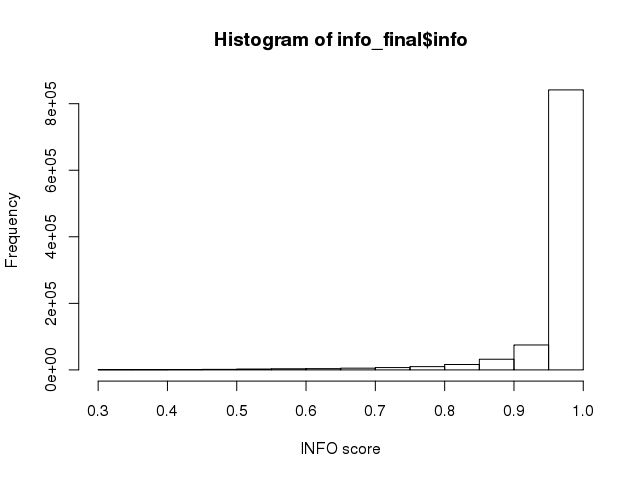
\includegraphics[width=\textwidth]{hist-simu1.png}
\caption{First simulations}
\label{fig:hist1}
\end{subfigure}
\begin{subfigure}[b]{0.45\textwidth}
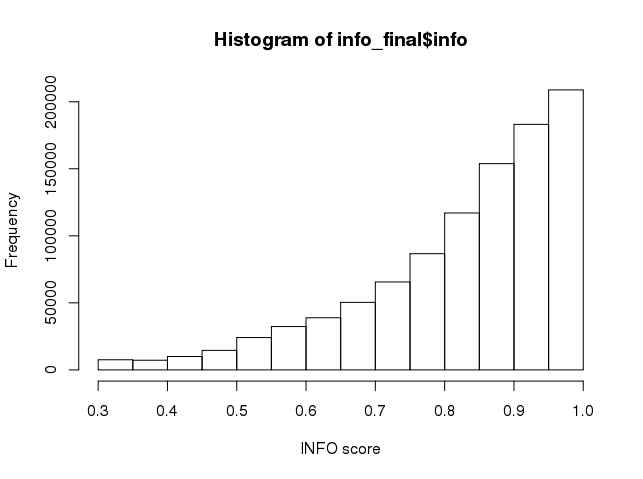
\includegraphics[width=\textwidth]{hist-simu2.png}
\caption{Second simulations}
\label{fig:hist2}
\end{subfigure}
\caption{Histogram of INFO scores for the 1M variants used in the simulations.}
\end{figure}

\vspace*{3em}

\begin{figure}[!htpb]
\centerline{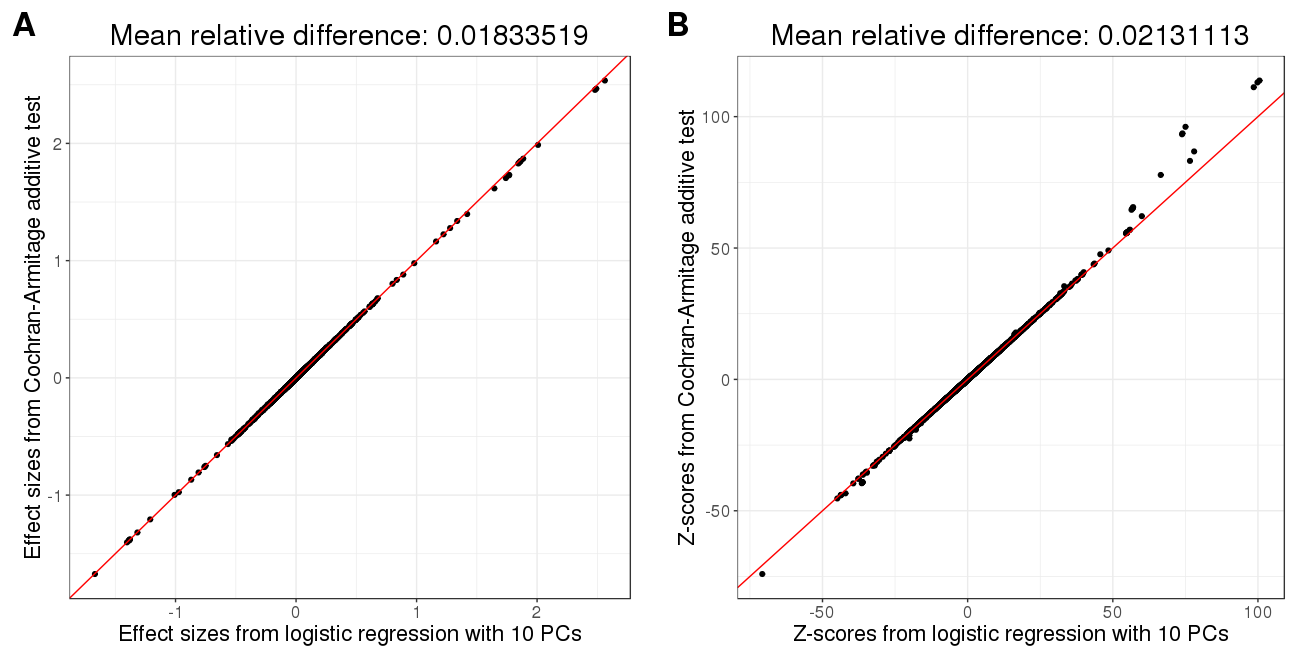
\includegraphics[width=0.9\textwidth]{equivalence.png}}
\caption{Comparison between logistic regression and Cochran-Armitage additive test. Comparison of estimated effect sizes (\textbf{A}) and Z-scores (\textbf{B}) if computed using a logistic regression with 10 principal components as covariates, or with a simple Cochran-Armitage additive test. Phenotypes were simulated using 100 causal variants only, allowing for large effects.}
\label{fig:GWAS}
\end{figure}

%%%%%%%%%%%%%%%%%%%%%%%%%%%%%%%%%%%%%%%%%%%%%%%%%%%%%%%%%%%%%%%%%%%%%%%%%%%%%%%%


\clearpage

\vspace*{1em}

\begin{figure}[!htpb]
\centerline{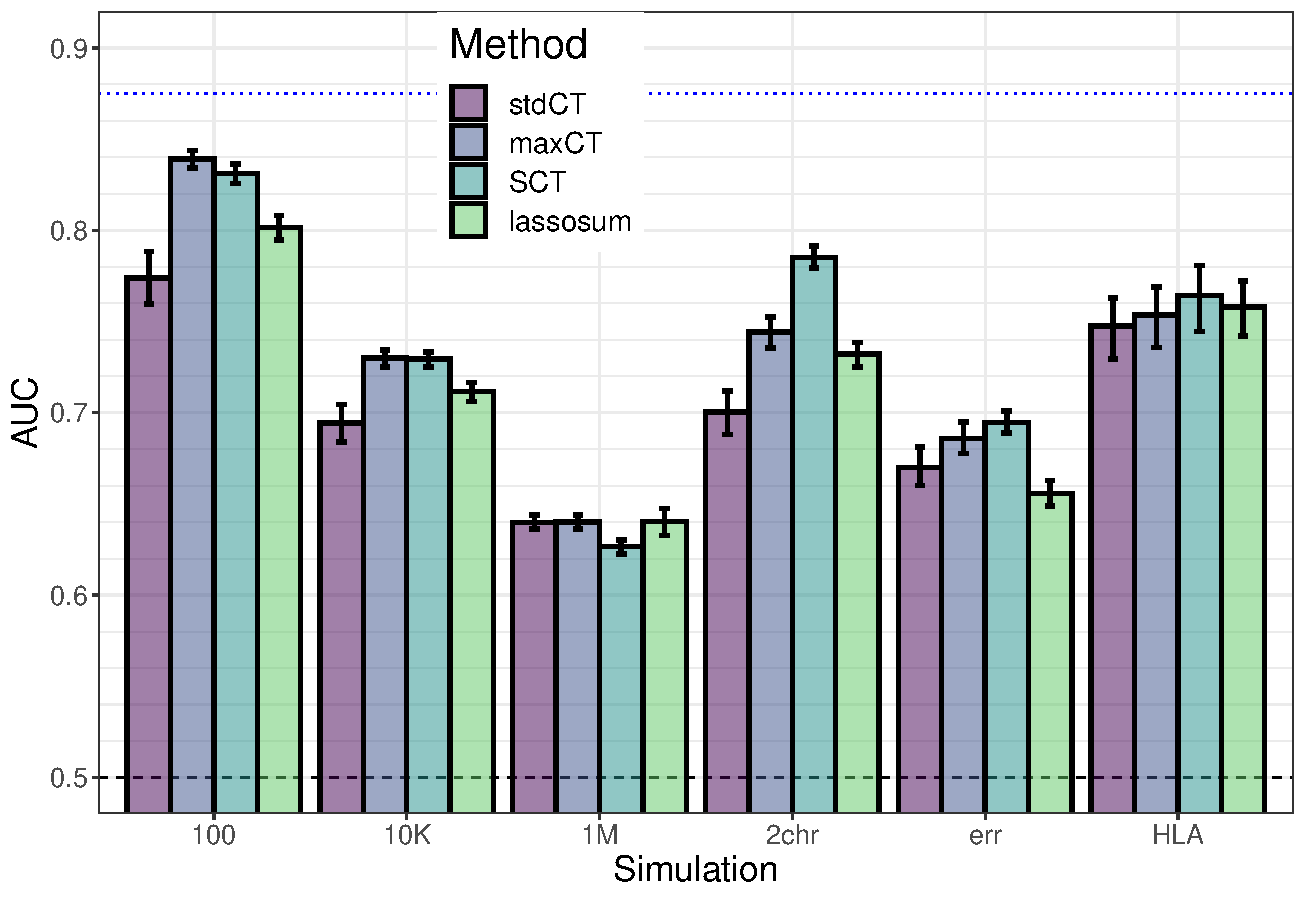
\includegraphics[width=0.8\textwidth]{AUC-simu2.pdf}}
\caption{Results of the 6 simulation scenarios with less well imputed variants. Scenarios are (100) 100 random causal variants; (10K) 10,000 random causal variants; (1M) all 1M variants are causal variants; (2chr) 100 variants of chromosome 1 are causal and all variants of chromosome 2, with half of the heritability for both chromosomes; (err) 10,000 random causal variants, but 10\% of the GWAS effects are reported with an opposite effect; (HLA) 7105 causal variants in a long-range LD region of chromosome 6. Mean and 95\% CI of $10^4$ non-parametric bootstrap replicates of the mean AUC of 10 simulations for each scenario. The blue dotted line represents the maximum achievable AUC for these simulations (87.5\% for a prevalence of 10\% and an heritability of 50\% -- see equation (3) of \cite{wray2010genetic}). See corresponding values in table \ref{tab:AUC-simu2}.}
\label{fig:AUC-simu2}
\end{figure}

%%%%%%%%%%%%%%%%%%%%%%%%%%%%%%%%%%%%%%%%%%%%%%%%%%%%%%%%%%%%%%%%%%%%%%%%%%%%%%%%

\clearpage
\vspace*{3em}

\begin{figure}[!htpb]
\centerline{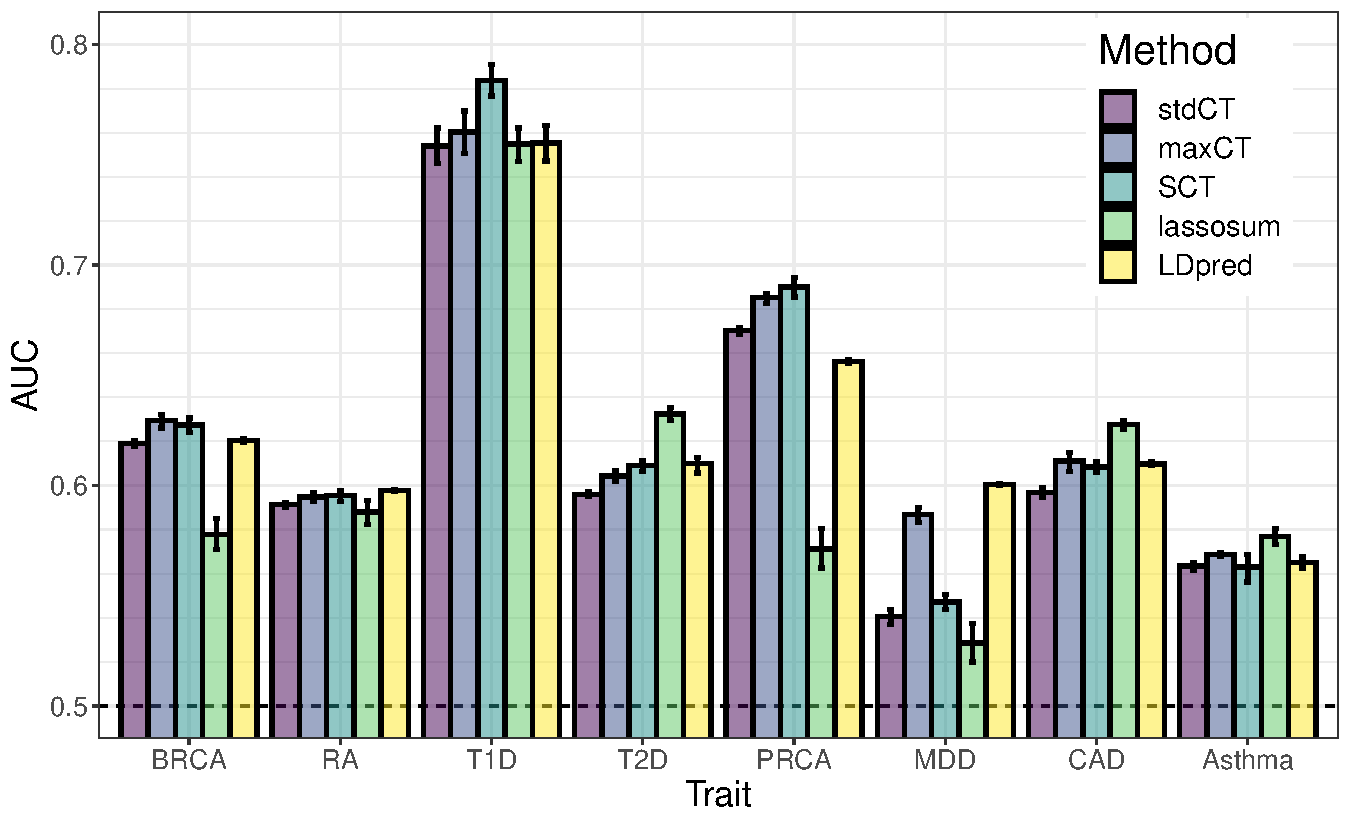
\includegraphics[width=0.8\textwidth]{AUC-real-small-mult.pdf}}
\caption{Results of the real data applications with small training size.
Mean and 95\% CI of $10^4$ non-parametric bootstrap replicates of the mean AUC of 6 random splits to define the training set. Training SCT and choosing optimal hyper-parameters for C+T, LDpred and lassosum use 500 cases and 2000 controls only. See corresponding values in table \ref{tab:AUC2}.}
\label{fig:AUC-real-small}
\end{figure}

\vspace*{4em}



%%%%%%%%%%%%%%%%%%%%%%%%%%%%%%%%%%%%%%%%%%%%%%%%%%%%%%%%%%%%%%%%%%%%%%%%%%%%%%%%

\begin{figure}[htbp]
\centering
\begin{subfigure}[b]{0.7\textwidth}
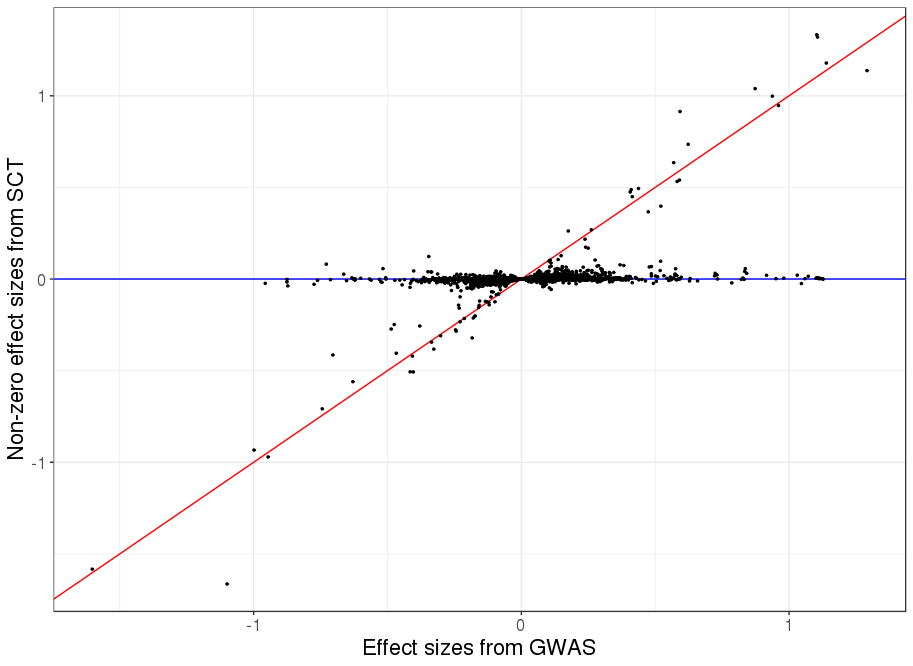
\includegraphics[width=\textwidth]{new-effects-simu100.png}
\caption{``100'': 100 random causal variants}
\end{subfigure}
\\~\\~\\
\begin{subfigure}[b]{0.7\textwidth}
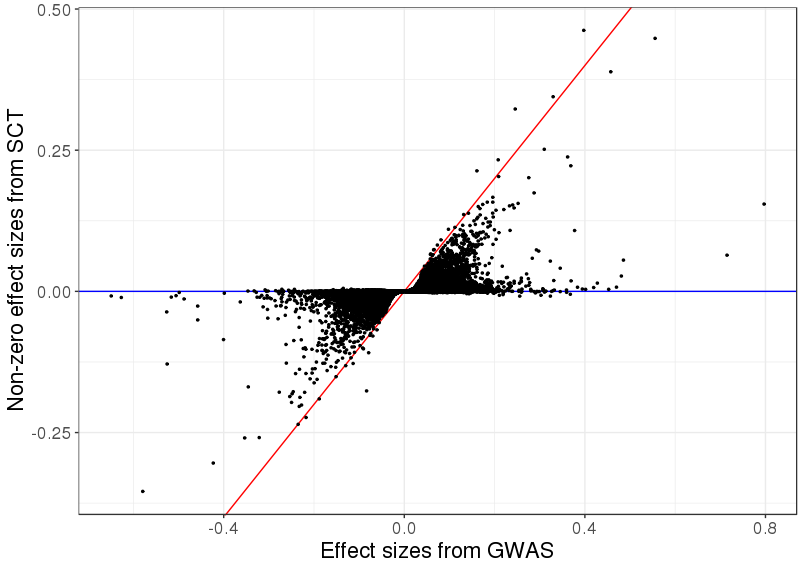
\includegraphics[width=\textwidth]{new-effects-simu10K.png}
\caption{``10K'': 10,000 random causal variants}
\end{subfigure}
\end{figure}

\begin{figure}[htb]\ContinuedFloat
\centering
\begin{subfigure}[b]{0.7\textwidth}
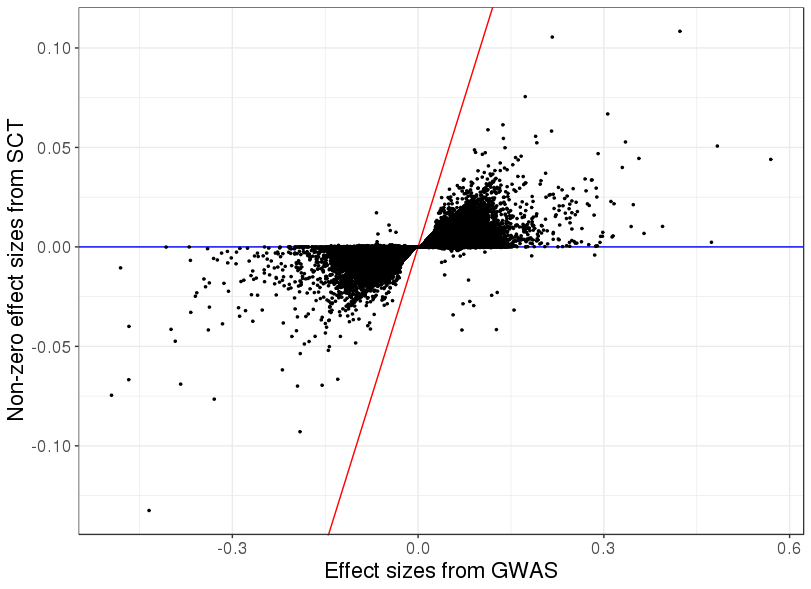
\includegraphics[width=\textwidth]{new-effects-simu1M.png}
\caption{``1M'': all 1M variants are causal variants\label{fig:neweff1M}}
\end{subfigure}
\\~\\~\\
\begin{subfigure}[b]{0.7\textwidth}
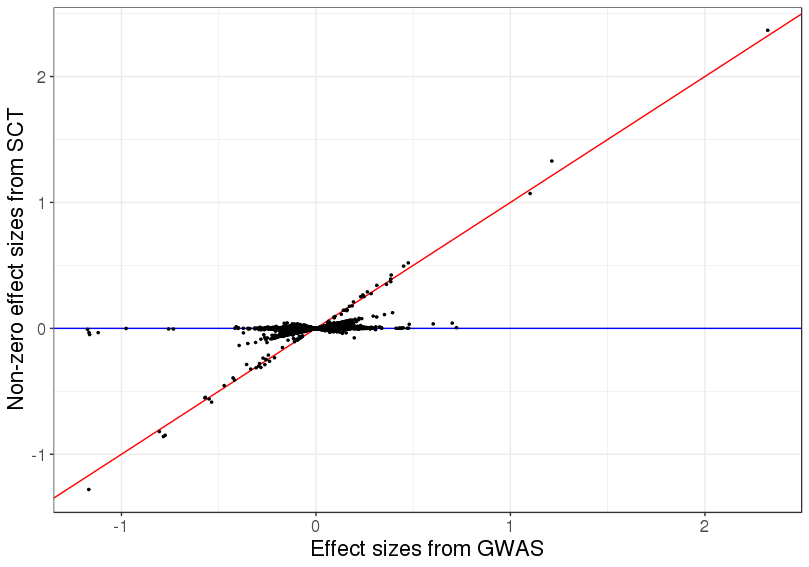
\includegraphics[width=\textwidth]{new-effects-simu2chr.png}
\caption{``2chr'': Causal variants on chromosomes 1 \& 2}
\end{subfigure}
\end{figure}

\begin{figure}[htb]\ContinuedFloat
\centering
\begin{subfigure}[b]{0.7\textwidth}
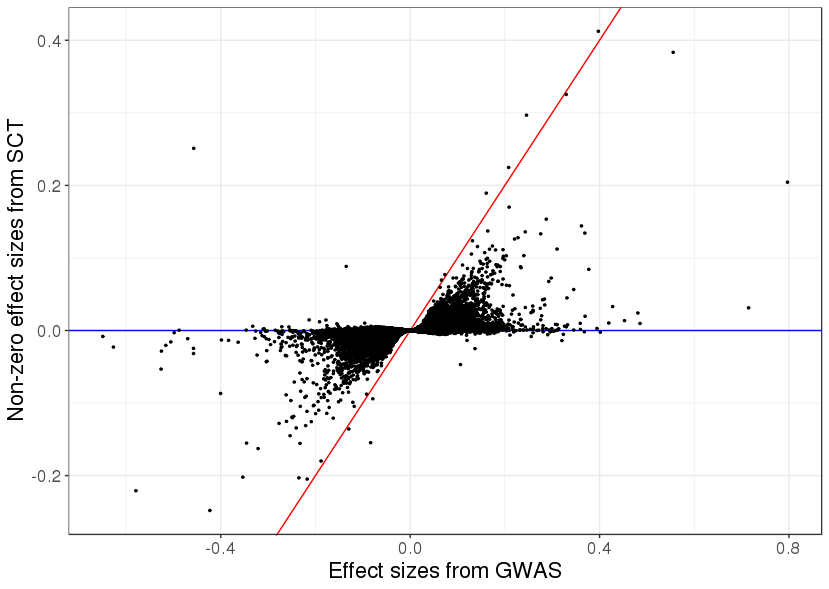
\includegraphics[width=\textwidth]{new-effects-simuerr.png}
\caption{``err'': 10,000 random causal variants, but 10\% of the GWAS effects are reported with an opposite effect\label{fig:newefferr}}
\end{subfigure}
\\~\\~\\
\begin{subfigure}[b]{0.7\textwidth}
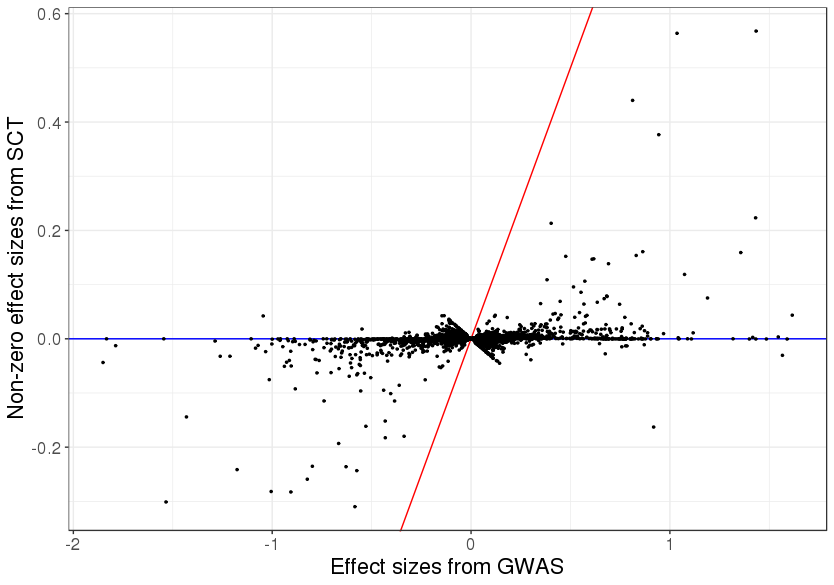
\includegraphics[width=\textwidth]{new-effects-simuHLA.png}
\caption{``HLA'': 7105 causal variants in a long-range LD region of chromosome 6\label{fig:neweffHLA}}
\end{subfigure}

\caption{Effect sizes in simulations. New effect sizes resulting from SCT versus initial effect sizes of GWAS in the first simulation of each simulation scenario. Only non-zero effects are represented. Red line corresponds to the 1:1 line.}
\label{fig:neweffsimu}
\end{figure}

%%%%%%%%%%%%%%%%%%%%%%%%%%%%%%%%%%%%%%%%%%%%%%%%%%%%%%%%%%%%%%%%%%%%%%%%%%%%%%%%

\begin{figure}[htb]
\centering
\begin{subfigure}[b]{\textwidth}
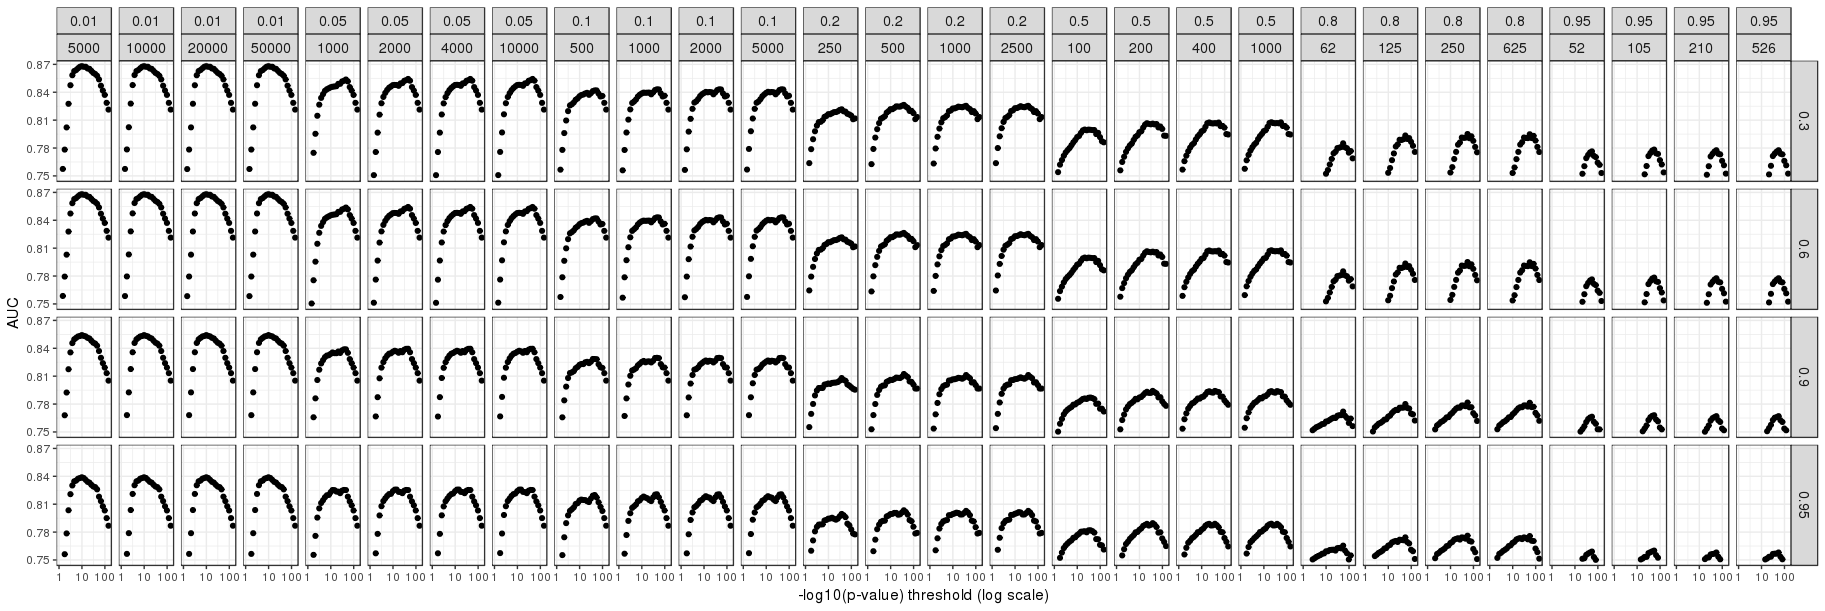
\includegraphics[width=\textwidth]{grid-simu100.png}
\caption{``100'': 100 random causal variants\label{fig:simugridA}}
\end{subfigure}
\\~\\~\\
\begin{subfigure}[b]{\textwidth}
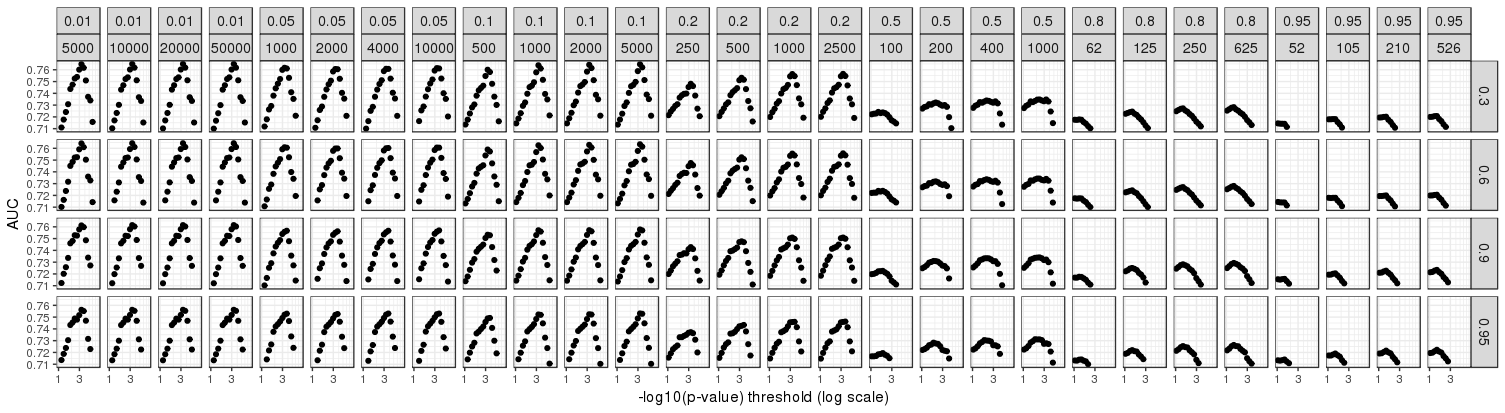
\includegraphics[width=\textwidth]{grid-simu10K.png}
\caption{``10K'': 10,000 random causal variants\label{fig:simugridB}}
\end{subfigure}
\\~\\~\\
\begin{subfigure}[b]{\textwidth}
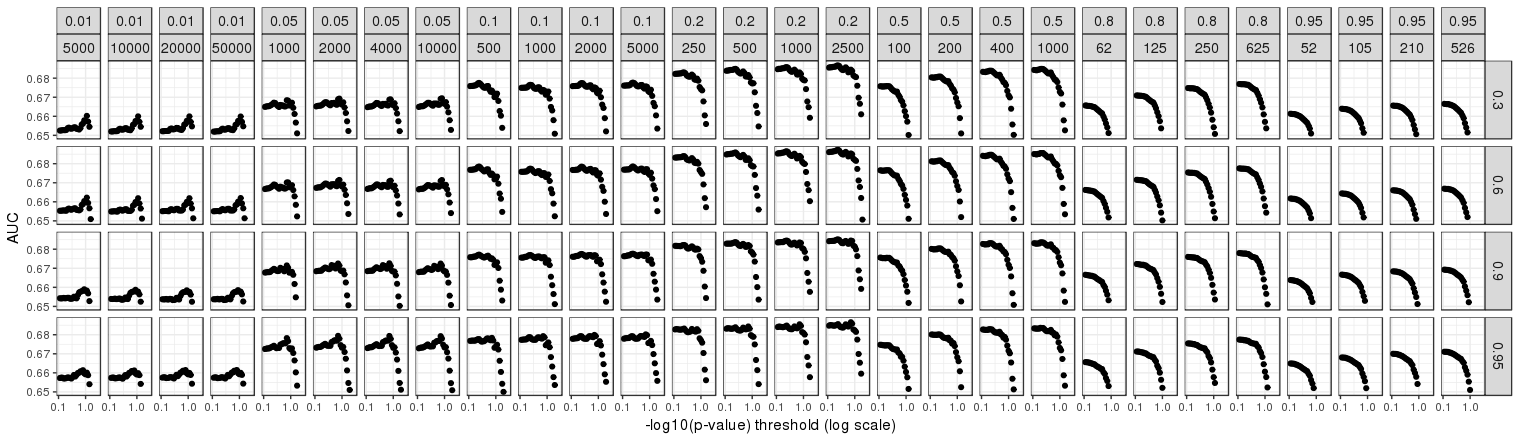
\includegraphics[width=\textwidth]{grid-simu1M.png}
\caption{``1M'': all 1M variants are causal variants\label{fig:simugridC}}
\end{subfigure}
\end{figure}

\begin{figure}[htb]\ContinuedFloat
\centering
\begin{subfigure}[b]{\textwidth}
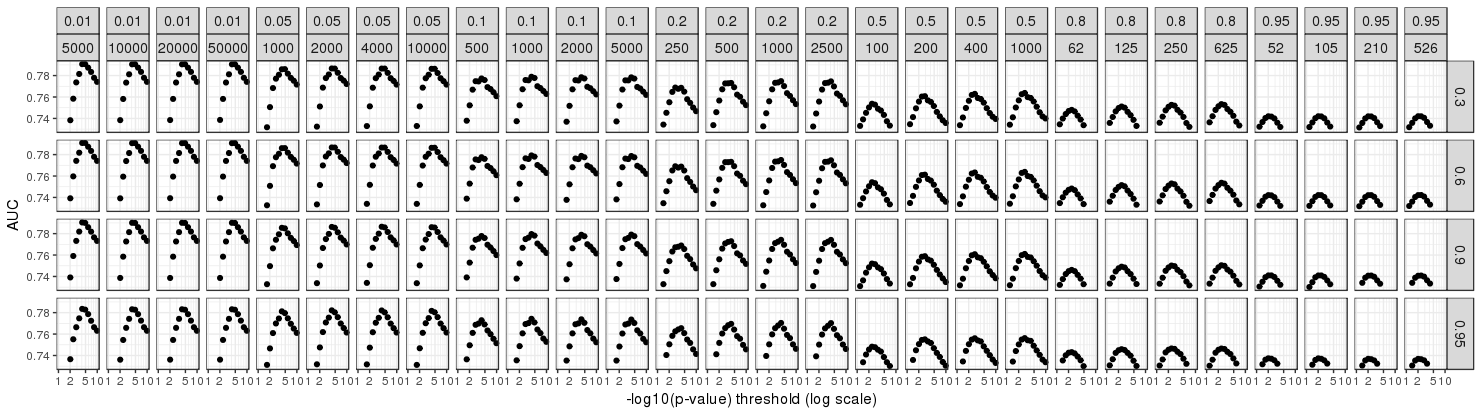
\includegraphics[width=\textwidth]{grid-simu2chr.png}
\caption{``2chr'': Causal variants on chromosomes 1 \& 2}
\end{subfigure}
\\~\\~\\
\begin{subfigure}[b]{\textwidth}
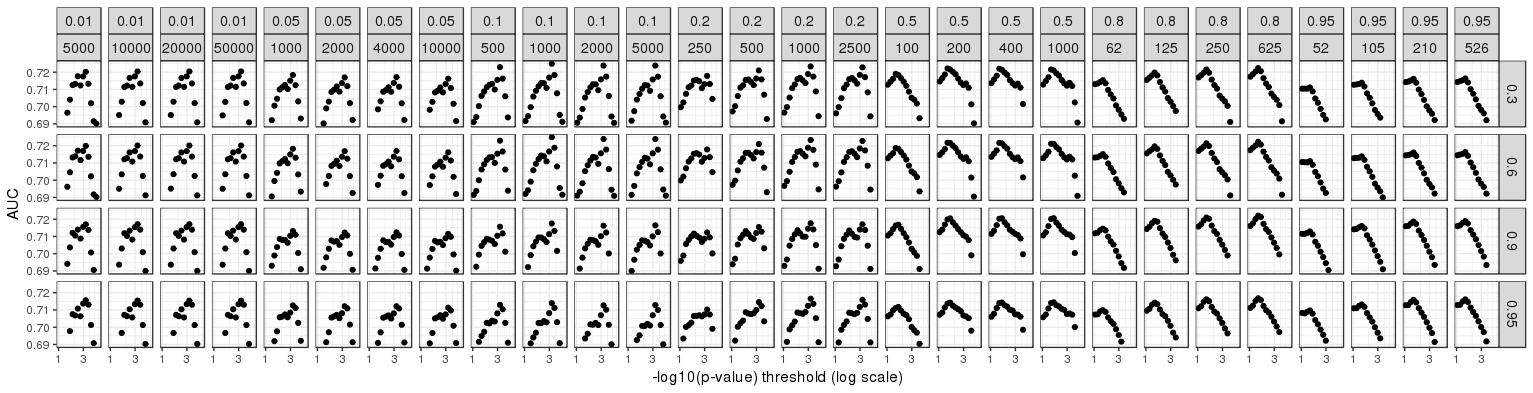
\includegraphics[width=\textwidth]{grid-simuerr.png}
\caption{``err'': 10,000 random causal variants, but 10\% of the GWAS effects are reported with an opposite effect}
\end{subfigure}
\\~\\~\\
\begin{subfigure}[b]{\textwidth}
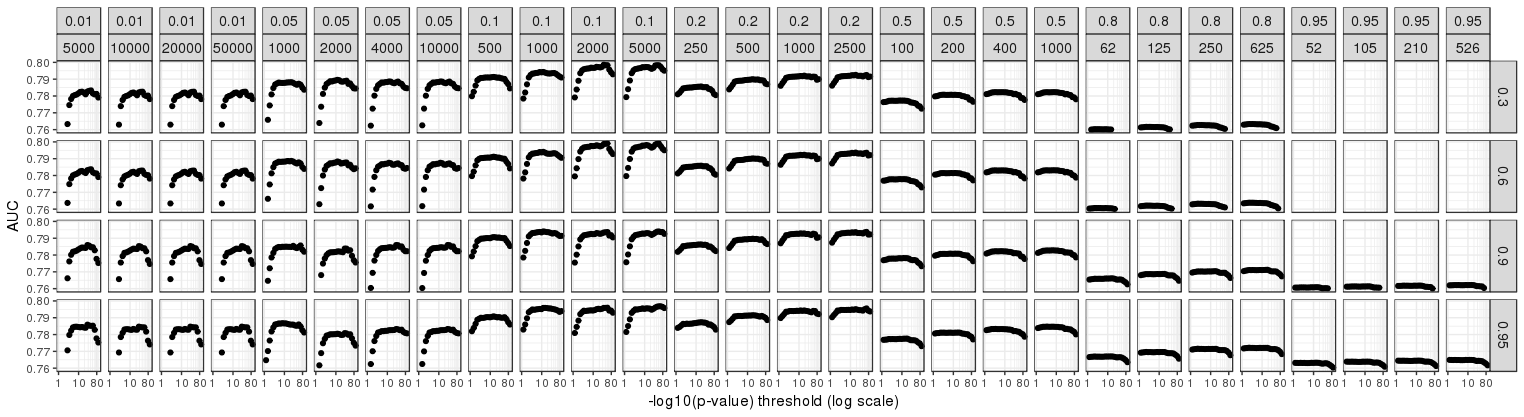
\includegraphics[width=\textwidth]{grid-simuHLA.png}
\caption{``HLA'': 7105 causal variants in a long-range LD region of chromosome 6}
\end{subfigure}

\caption{AUC results of all C+T scores in simulations with well imputed variants. AUC values (for the training set) when predicting disease status for many parameters of C+T in the first simulation of each simulation scenario when using well imputed variants. Facets are presenting different clumping thresholds $r_c^2$ from 0.01 to 0.95, window sizes $w_c$ from 52 to 50,000 kb, and imputation thresholds from 0.3 to 0.95. The x-axis corresponds to the remaining hyper-parameter, the p-value threshold $p_T$; here, -log10(p-values) are represented using a logarithmic scale.\label{fig:simu1grid}}
\end{figure}


\begin{figure}[htb]
\centering
\begin{subfigure}[b]{\textwidth}
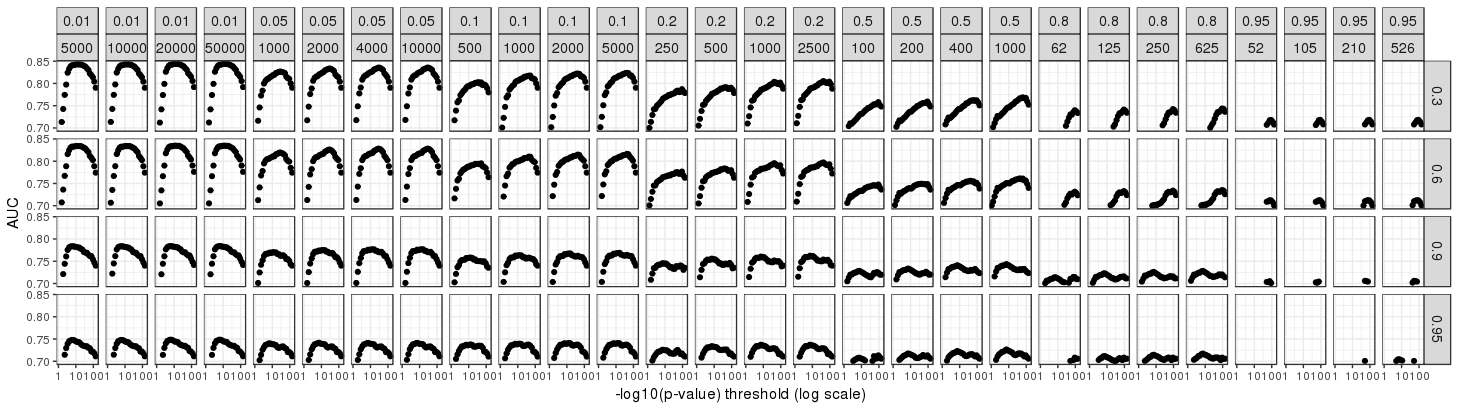
\includegraphics[width=\textwidth]{grid-simu100-2.png}
\caption{``100'': 100 random causal variants}
\end{subfigure}
\\~\\~\\
\begin{subfigure}[b]{\textwidth}
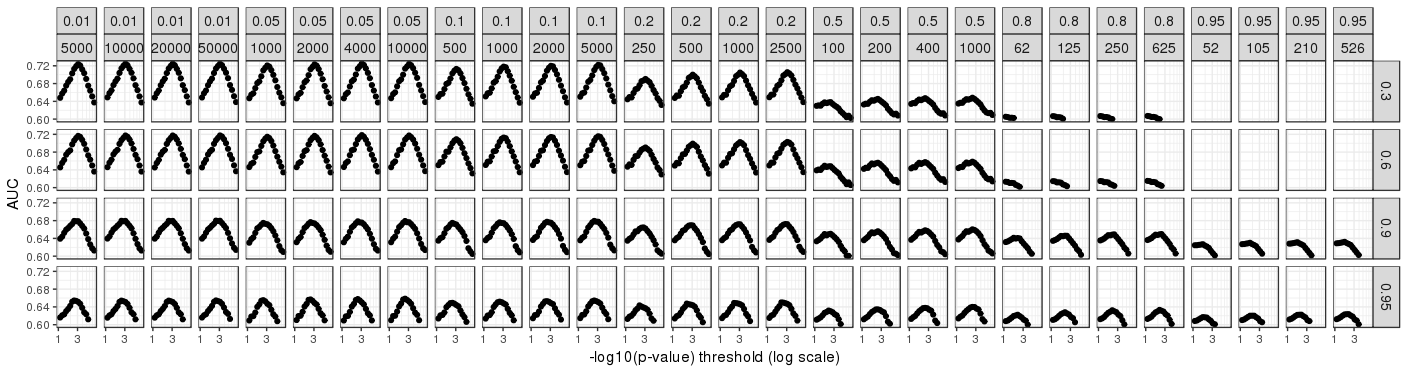
\includegraphics[width=\textwidth]{grid-simu10K-2.png}
\caption{``10K'': 10,000 random causal variants}
\end{subfigure}
\\~\\~\\
\begin{subfigure}[b]{\textwidth}
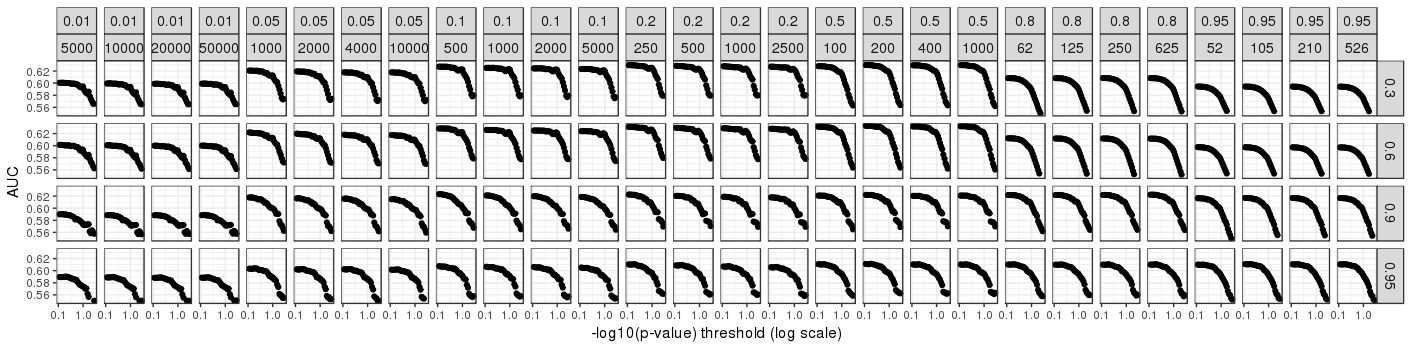
\includegraphics[width=\textwidth]{grid-simu1M-2.png}
\caption{``1M'': all 1M variants are causal variants}
\end{subfigure}
\end{figure}

\begin{figure}[htb]\ContinuedFloat
\centering
\begin{subfigure}[b]{\textwidth}
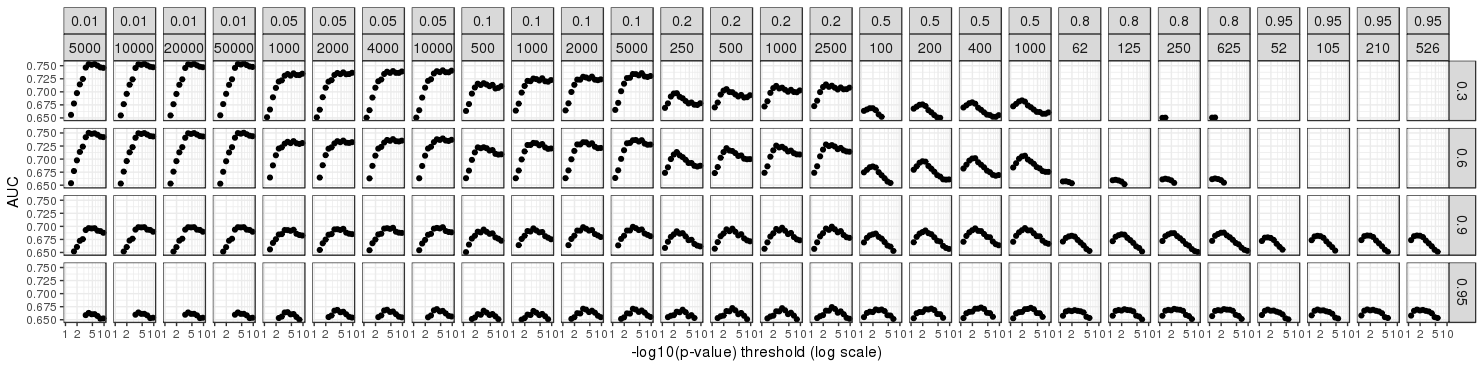
\includegraphics[width=\textwidth]{grid-simu2chr-2.png}
\caption{``2chr'': Causal variants on chromosomes 1 \& 2}
\end{subfigure}
\\~\\~\\
\begin{subfigure}[b]{\textwidth}
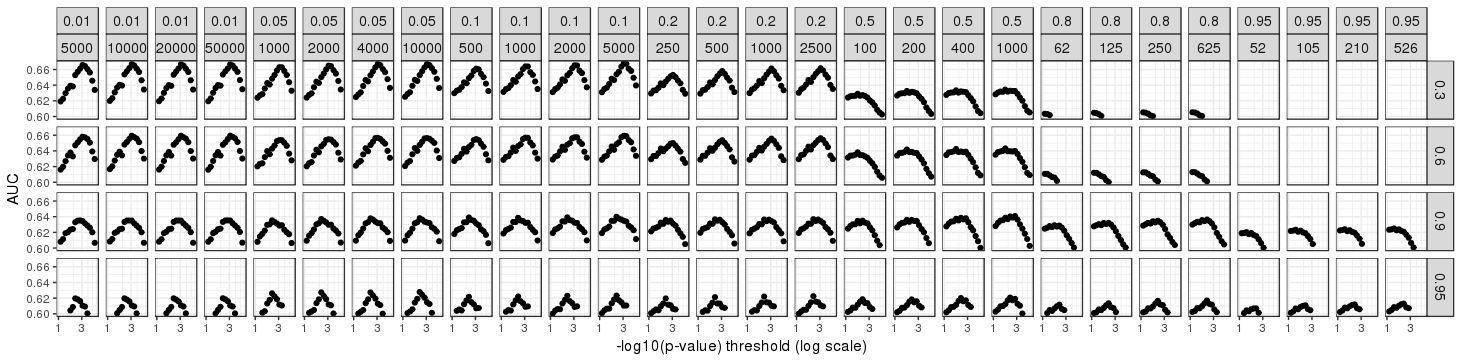
\includegraphics[width=\textwidth]{grid-simuerr-2.png}
\caption{``err'': 10,000 random causal variants, but 10\% of the GWAS effects are reported with an opposite effect}
\end{subfigure}
\\~\\~\\
\begin{subfigure}[b]{\textwidth}
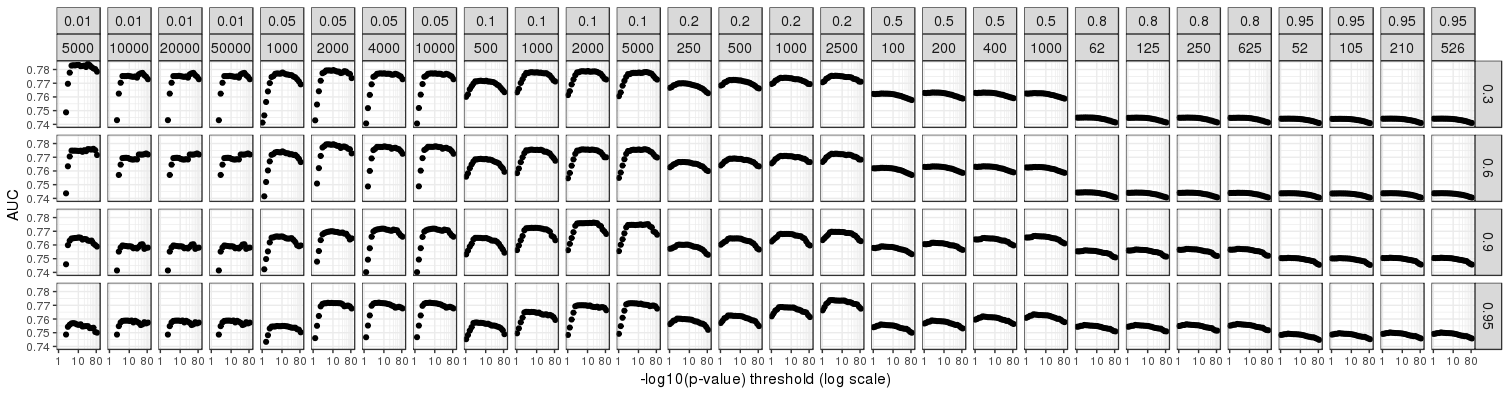
\includegraphics[width=\textwidth]{grid-simuHLA-2.png}
\caption{``HLA'': 7105 causal variants in a long-range LD region of chromosome 6}
\end{subfigure}

\caption{AUC results of all C+T scores in simulations with less well imputed variants. AUC values (for the training set) when predicting disease status for many parameters of C+T in the first simulation of each simulation scenario when using less well imputed variants. Facets are presenting different clumping thresholds $r_c^2$ from 0.01 to 0.95, window sizes $w_c$ from 52 to 50,000 kb, and imputation thresholds from 0.3 to 0.95. The x-axis corresponds to the remaining hyper-parameter, the p-value threshold $p_T$; here, -log10(p-values) are represented using a logarithmic scale.\label{fig:simu2grid}}
\end{figure}

%%%%%%%%%%%%%%%%%%%%%%%%%%%%%%%%%%%%%%%%%%%%%%%%%%%%%%%%%%%%%%%%%%%%%%%%%%%%%%%%

\begin{figure}[htb]
\centering
\begin{subfigure}[b]{0.7\textwidth}
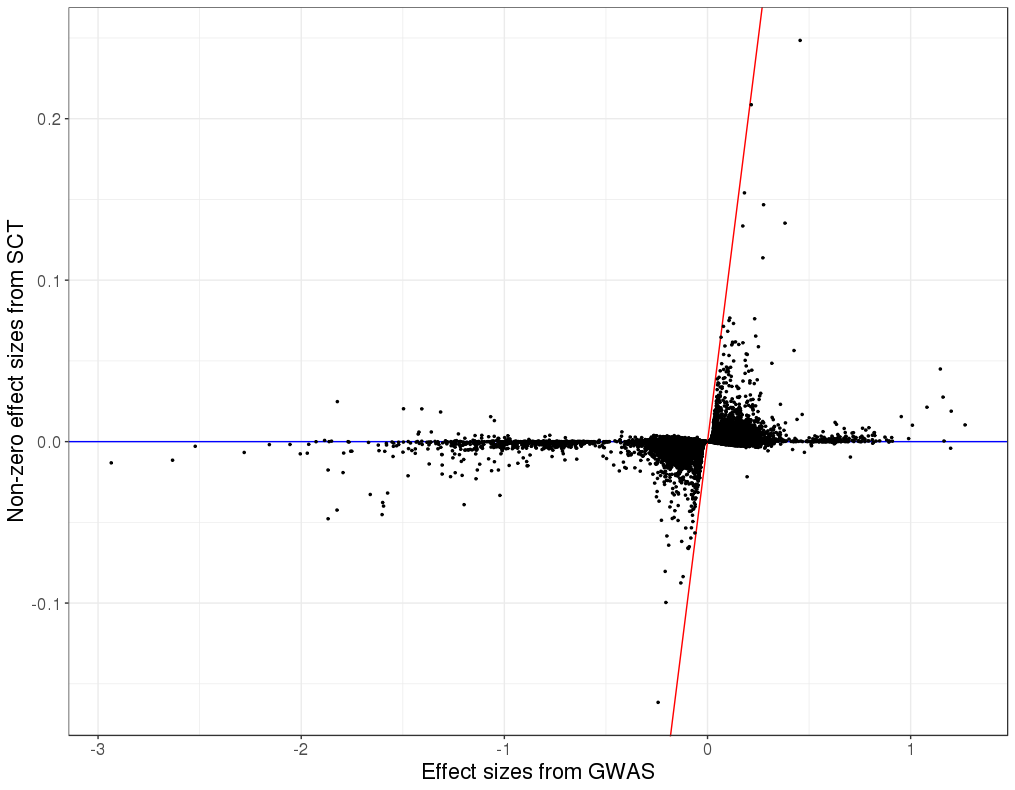
\includegraphics[width=\textwidth]{new-effects-BRCA.png}
\caption{Breast cancer}
\end{subfigure}
\\~\\~\\
\begin{subfigure}[b]{0.7\textwidth}
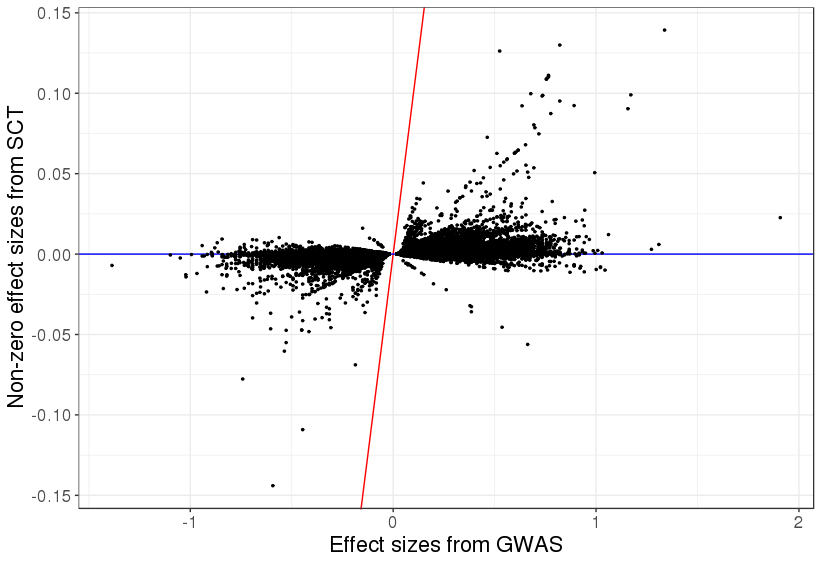
\includegraphics[width=\textwidth]{new-effects-RA.png}
\caption{Rheumatoid arthritis}
\end{subfigure}
\end{figure}

\begin{figure}[htb]\ContinuedFloat
\centering
\begin{subfigure}[b]{0.7\textwidth}
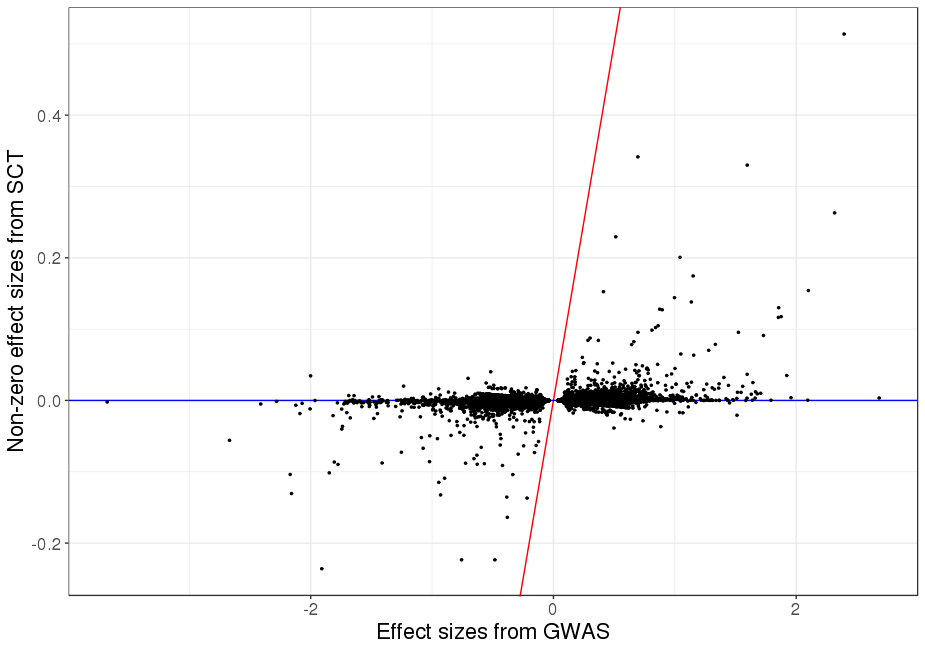
\includegraphics[width=\textwidth]{new-effects-T1D.png}
\caption{Type 1 diabetes}
\end{subfigure}
\\~\\~\\
\begin{subfigure}[b]{0.7\textwidth}
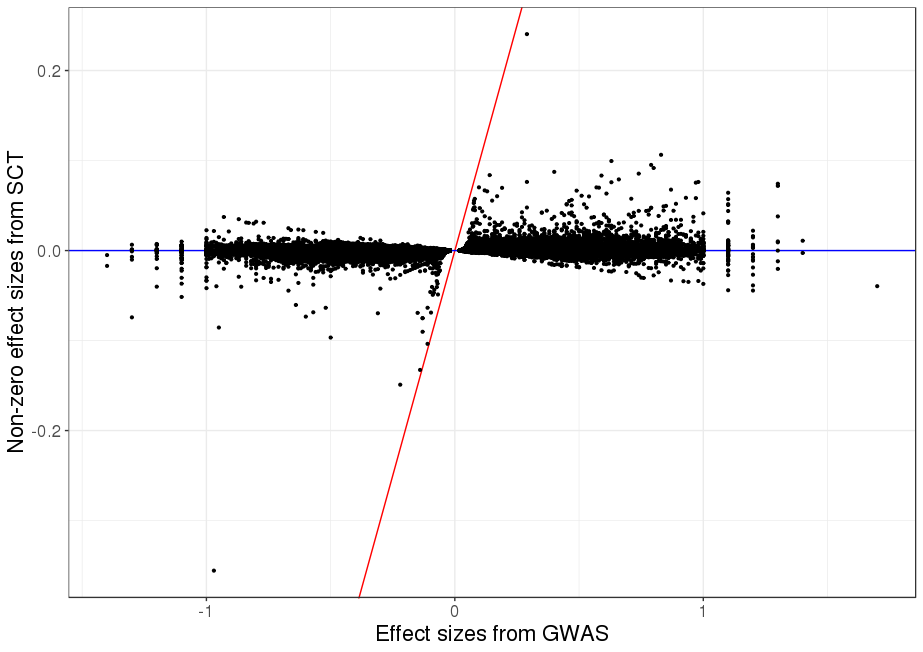
\includegraphics[width=\textwidth]{new-effects-T2D.png}
\caption{Type 2 diabetes}
\end{subfigure}
\end{figure}

\begin{figure}[htb]\ContinuedFloat
\centering
\begin{subfigure}[b]{0.7\textwidth}
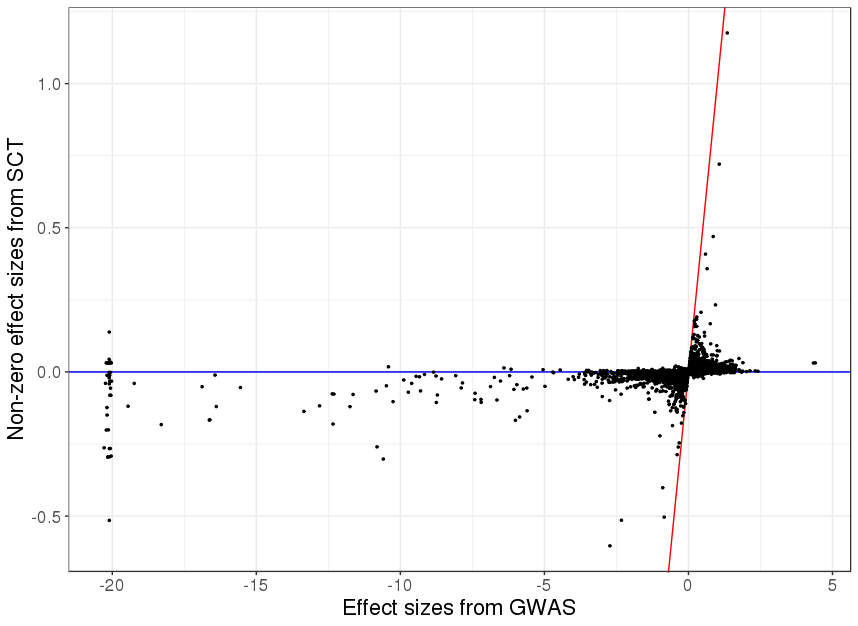
\includegraphics[width=\textwidth]{new-effects-PRCA.png}
\caption{Prostate cancer}
\end{subfigure}
\\~\\~\\
\begin{subfigure}[b]{0.7\textwidth}
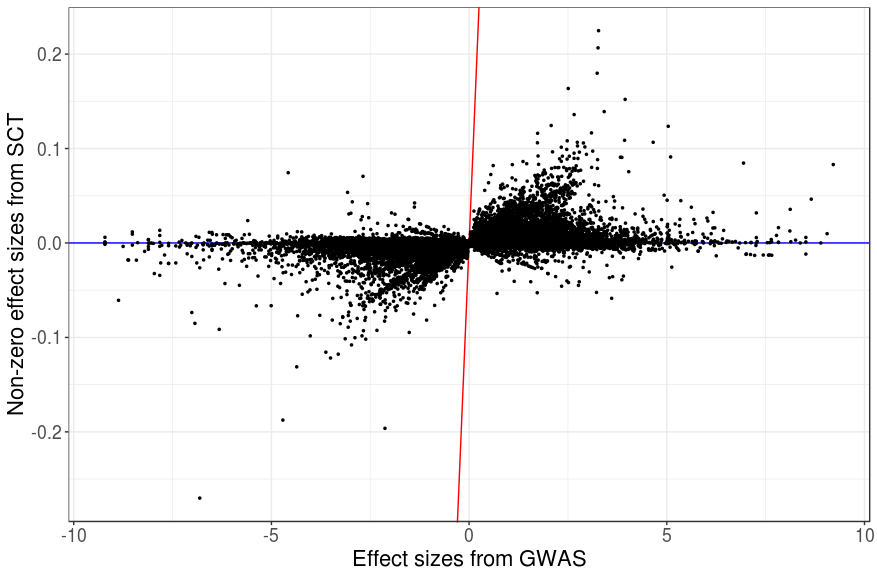
\includegraphics[width=\textwidth]{new-effects-MDD.png}
\caption{Depression}
\end{subfigure}
\end{figure}

\begin{figure}[htb]\ContinuedFloat
\centering
\begin{subfigure}[b]{0.7\textwidth}
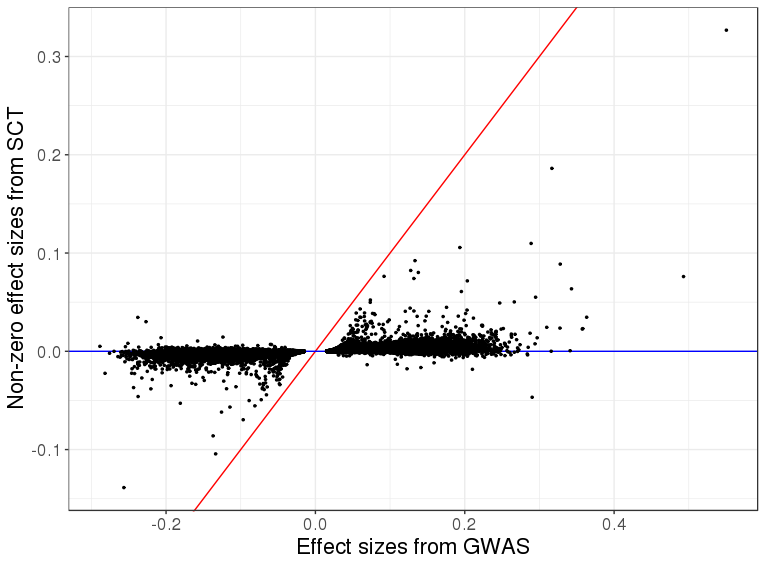
\includegraphics[width=\textwidth]{new-effects-CAD.png}
\caption{Coronary artery disease}
\end{subfigure}
\\~\\~\\
\begin{subfigure}[b]{0.7\textwidth}
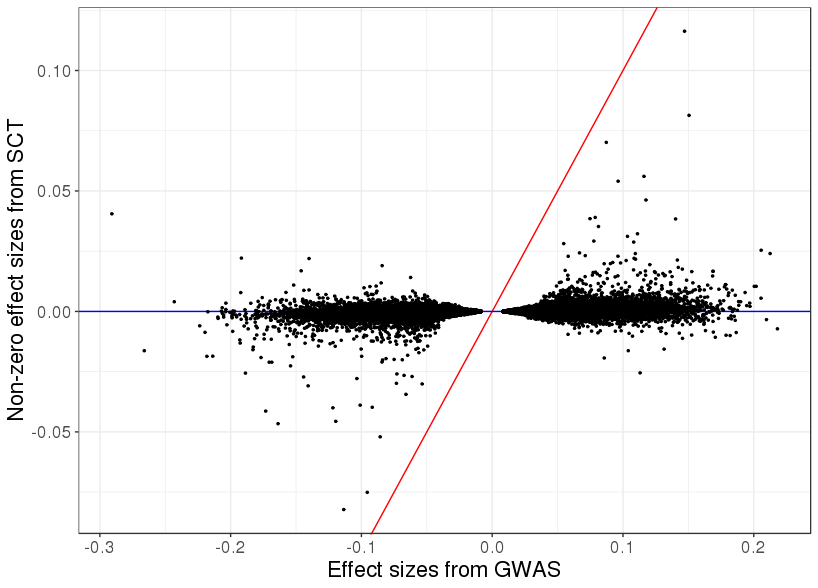
\includegraphics[width=\textwidth]{new-effects-asthma.png}
\caption{Asthma}
\end{subfigure}

\caption{Effect sizes in real data applications. New effect sizes resulting from SCT versus initial effect sizes of GWAS in real data applications. Only non-zero effects are represented. Red line corresponds to the 1:1 line.}
\label{fig:neweffreal}
\end{figure}

%%%%%%%%%%%%%%%%%%%%%%%%%%%%%%%%%%%%%%%%%%%%%%%%%%%%%%%%%%%%%%%%%%%%%%%%%%%%%%%%

\begin{figure}[htb]
\centering
\begin{subfigure}[b]{\textwidth}
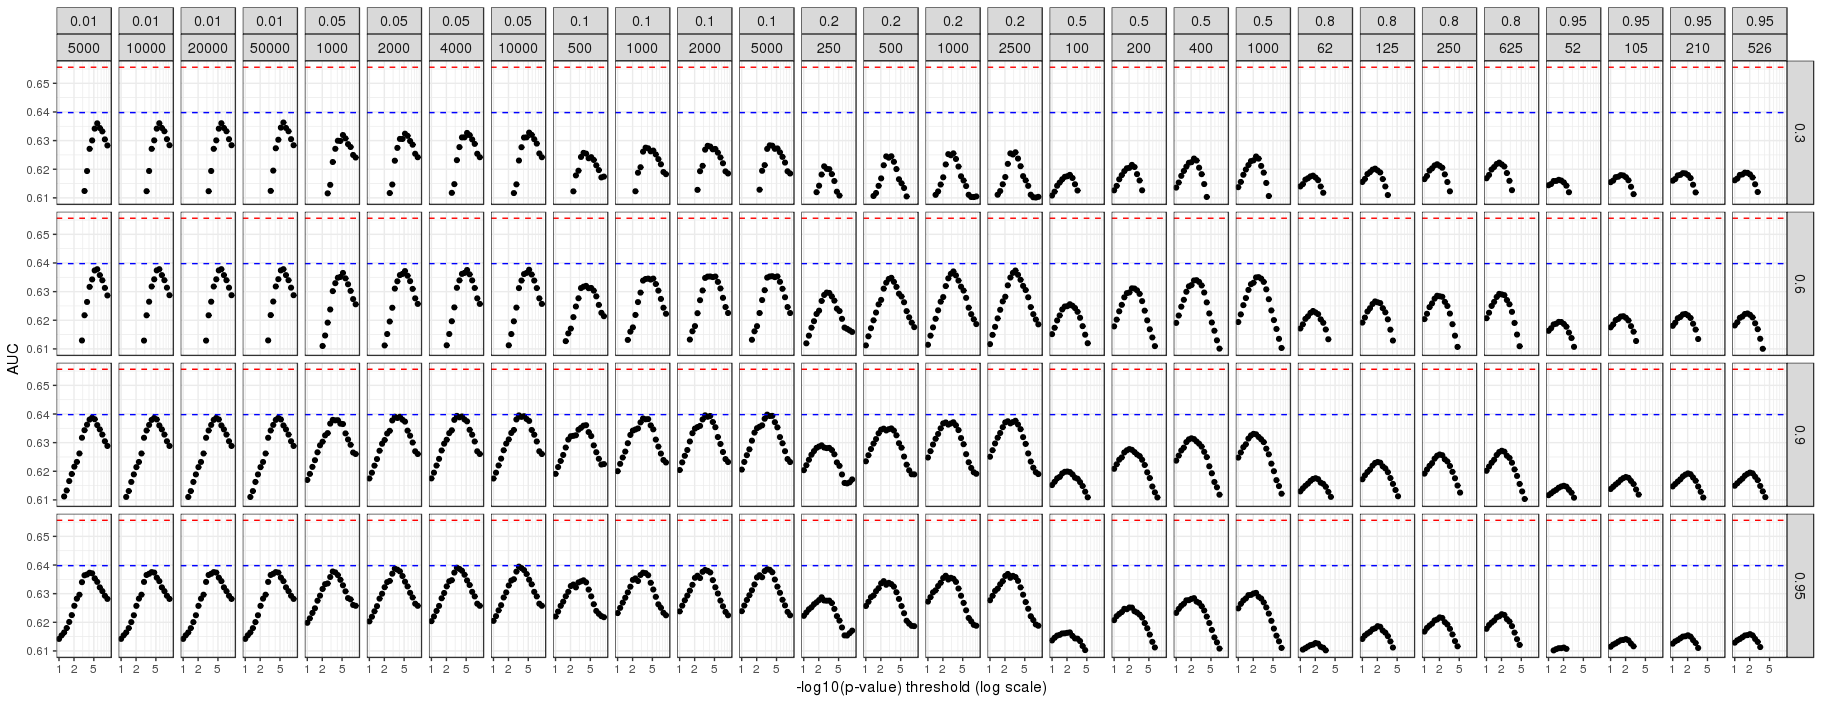
\includegraphics[width=\textwidth]{grid-BRCA.png}
\caption{Breast cancer}
\end{subfigure}
\\~\\
\begin{subfigure}[b]{\textwidth}
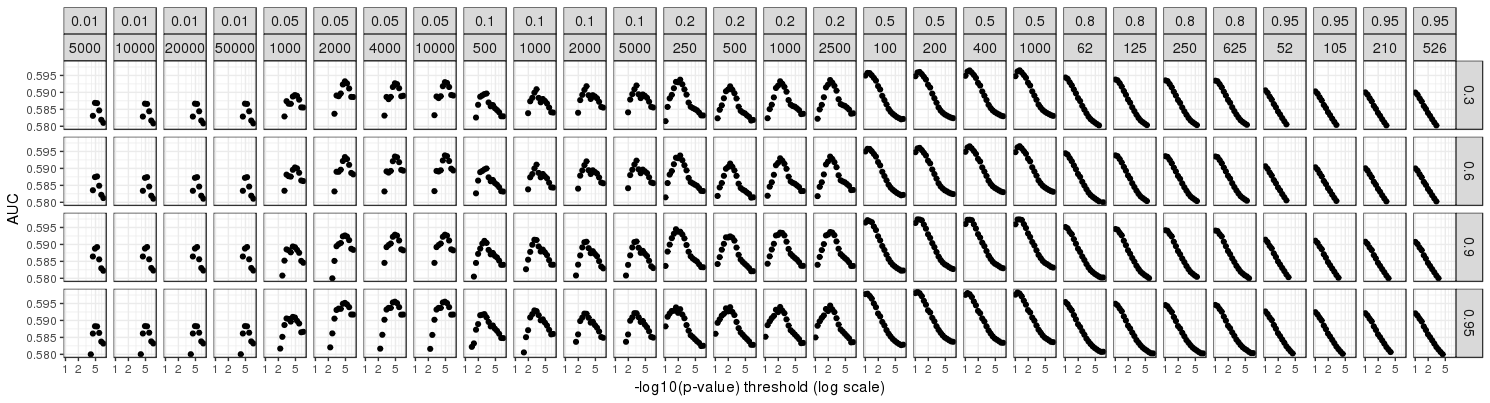
\includegraphics[width=\textwidth]{grid-RA.png}
\caption{Rheumatoid arthritis\label{fig:grid-RA}}
\end{subfigure}
\\~\\
\begin{subfigure}[b]{\textwidth}
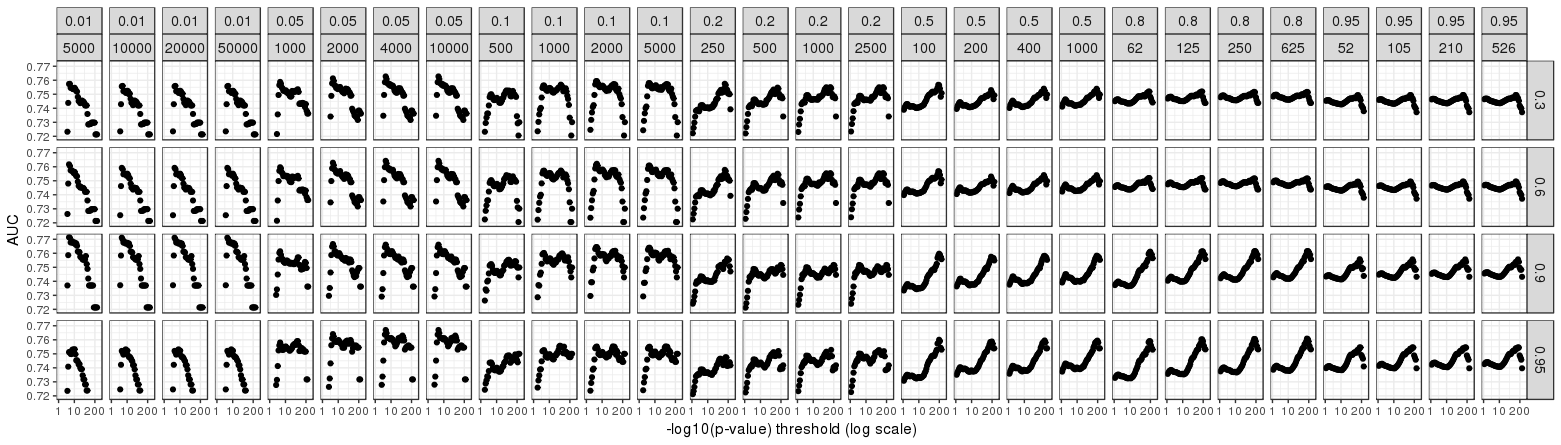
\includegraphics[width=\textwidth]{grid-T1D.png}
\caption{Type 1 diabetes}
\end{subfigure}
\end{figure}

\begin{figure}[htb]\ContinuedFloat
\centering
\begin{subfigure}[b]{\textwidth}
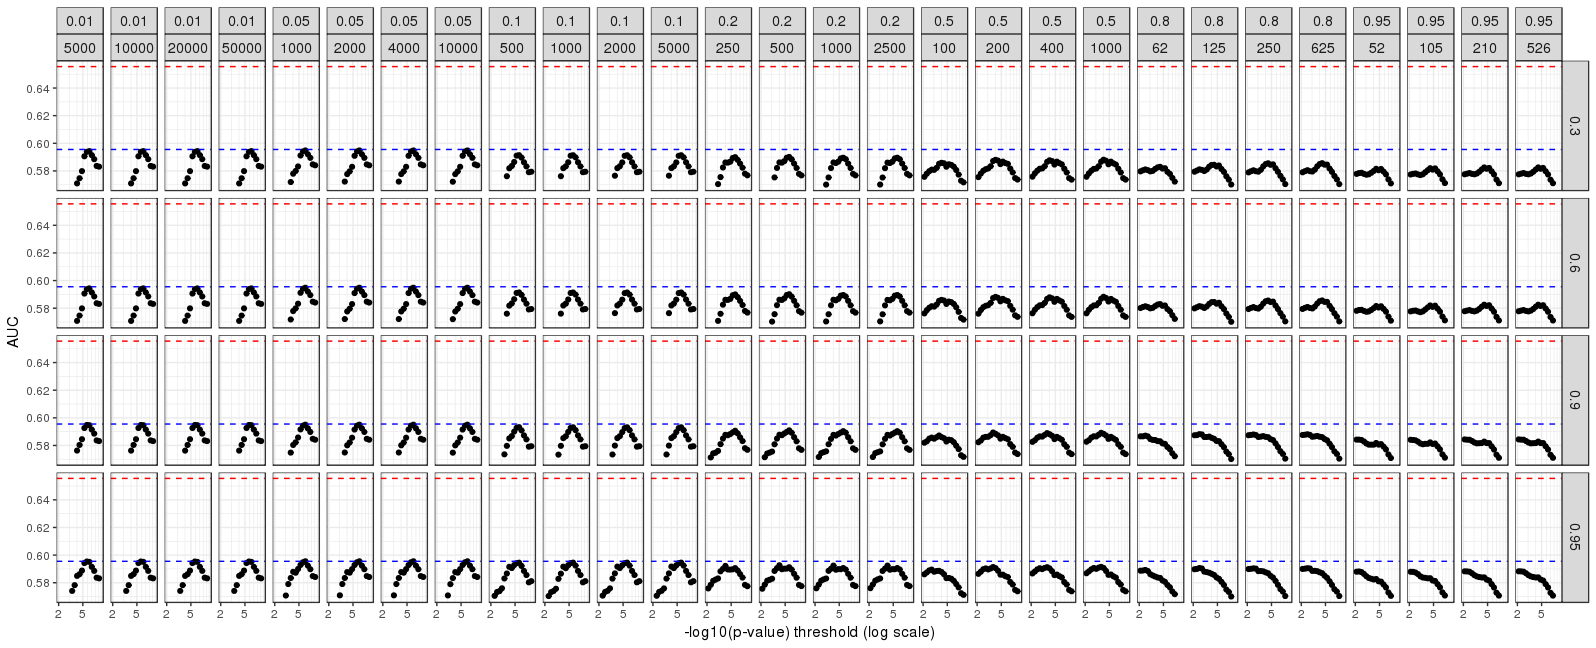
\includegraphics[width=\textwidth]{grid-T2D.png}
\caption{Type 2 diabetes}
\end{subfigure}
\\~\\
\begin{subfigure}[b]{\textwidth}
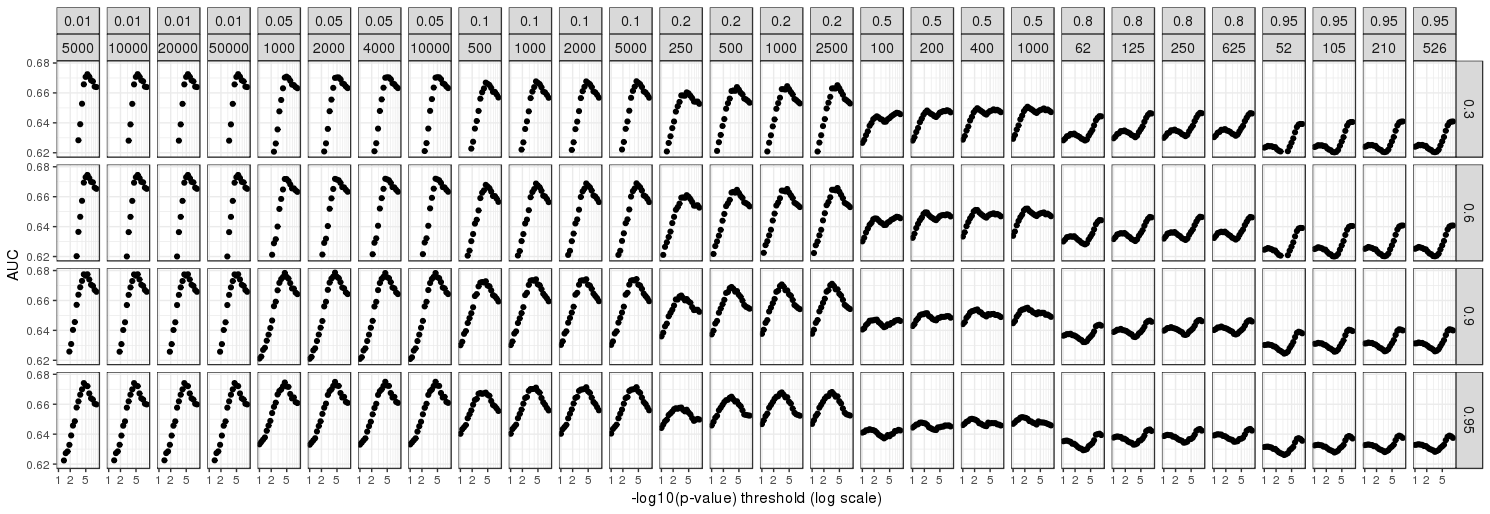
\includegraphics[width=\textwidth]{grid-PRCA.png}
\caption{Prostate cancer}
\end{subfigure}
\\~\\
\begin{subfigure}[b]{\textwidth}
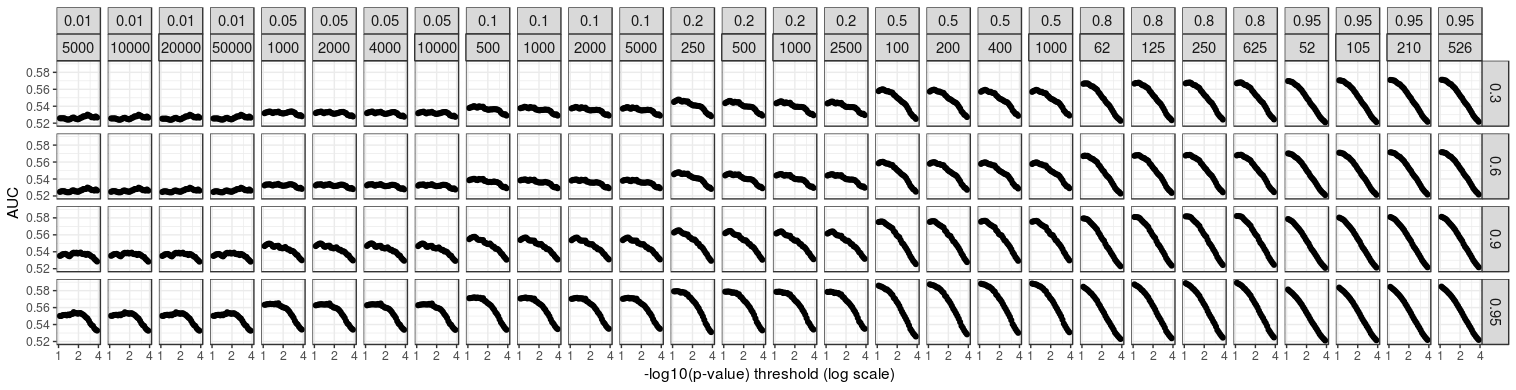
\includegraphics[width=\textwidth]{grid-MDD.png}
\caption{Depression\label{fig:grid-MDD}}
\end{subfigure}
\end{figure}

\begin{figure}[htb]\ContinuedFloat
\centering
\begin{subfigure}[b]{\textwidth}
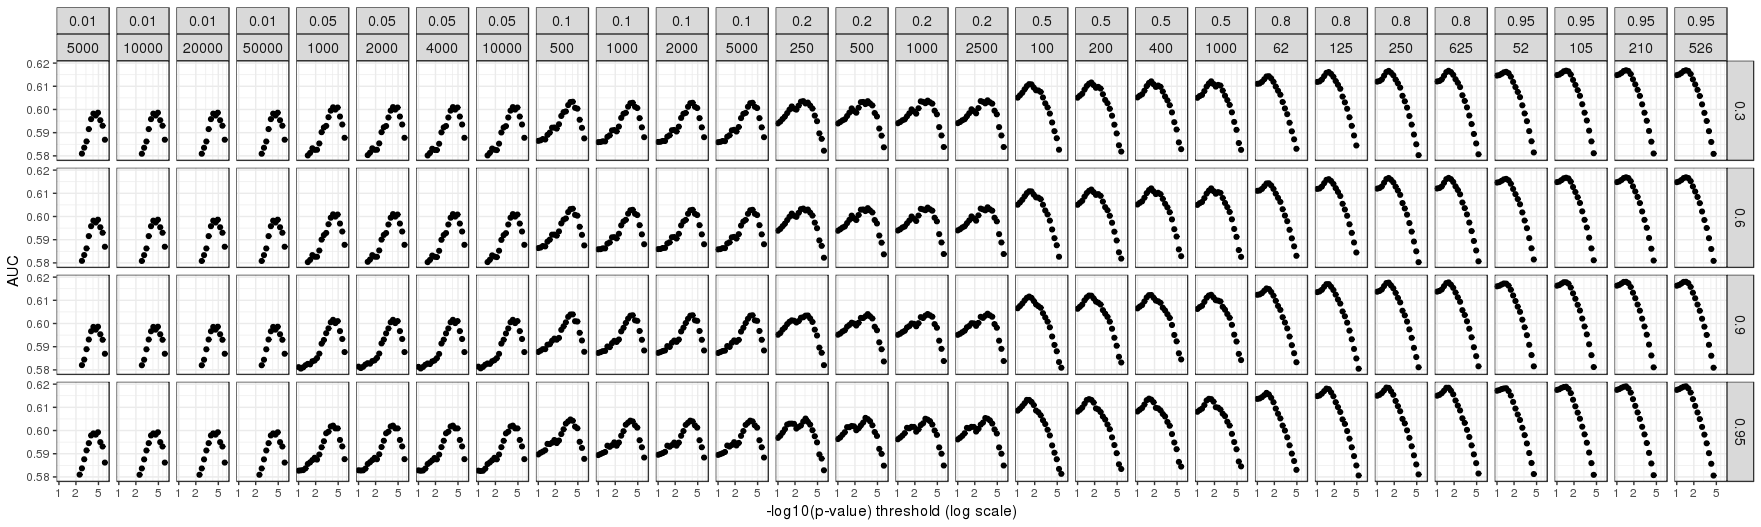
\includegraphics[width=\textwidth]{grid-CAD.png}
\caption{Coronary artery disease\label{fig:grid-CAD}}
\end{subfigure}
\\~\\
\begin{subfigure}[b]{\textwidth}
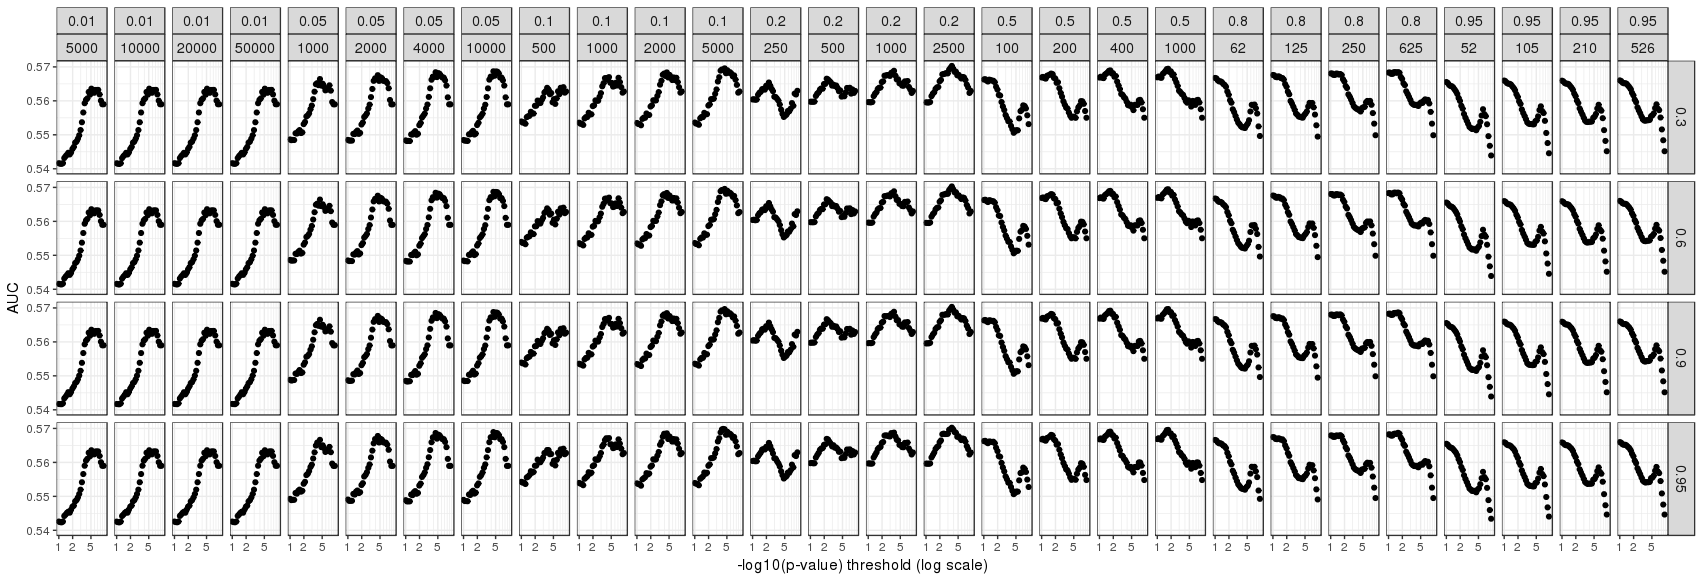
\includegraphics[width=\textwidth]{grid-asthma.png}
\caption{Asthma}
\end{subfigure}

\caption{AUC results of all C+T scores in real data applications.
AUC values (for the training set) when predicting disease status for many parameters of C+T in real data applications. Facets are presenting different clumping thresholds $r_c^2$ from 0.01 to 0.95, window sizes $w_c$ from 52 to 50,000 kb, and imputation thresholds from 0.3 to 0.95. The x-axis corresponds to the remaining hyper-parameter, the p-value threshold $p_T$; here, -log10(p-values) are represented using a logarithmic scale.}
\end{figure}

%%%%%%%%%%%%%%%%%%%%%%%%%%%%%%%%%%%%%%%%%%%%%%%%%%%%%%%%%%%%%%%%%%%%%%%%%%%%%%%%

\begin{figure}[htb]
\centering
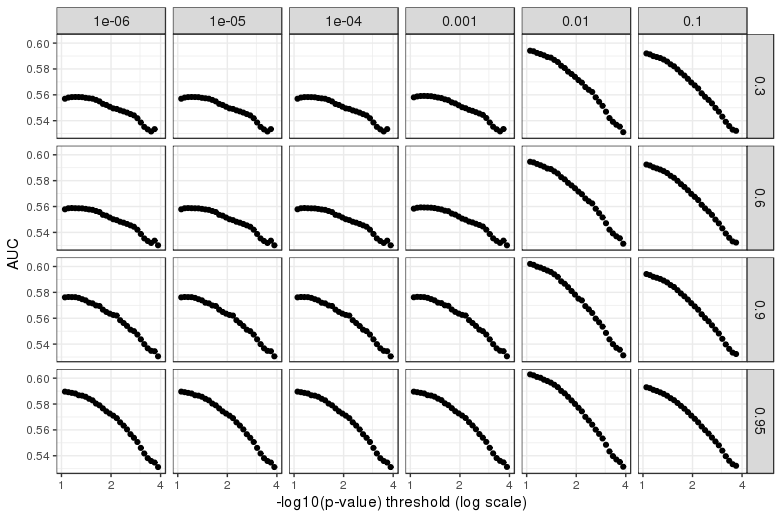
\includegraphics[width=\textwidth]{grid-MDD-with-MAF.png}
\caption{AUC results of all C+T scores for MDD when including MAF. 
AUC values (for the training set) when predicting MDD status for many parameters of C+T in real data application. Facets are presenting different MAF thresholds (top), and imputation thresholds from 0.3 to 0.95 (right). Parameter $r_c^2$ was fixed at 0.5 and $w_c$ at 1000 kb. The x-axis corresponds to the remaining hyper-parameter, the p-value threshold $p_T$; here, -log10(p-values) are represented using a logarithmic scale.\label{fig:grid-MAF}}
\end{figure}

%%%%%%%%%%%%%%%%%%%%%%%%%%%%%%%%%%%%%%%%%%%%%%%%%%%%%%%%%%%%%%%%%%%%%%%%%%%%%%%%

\begin{figure}[htb]
\centerline{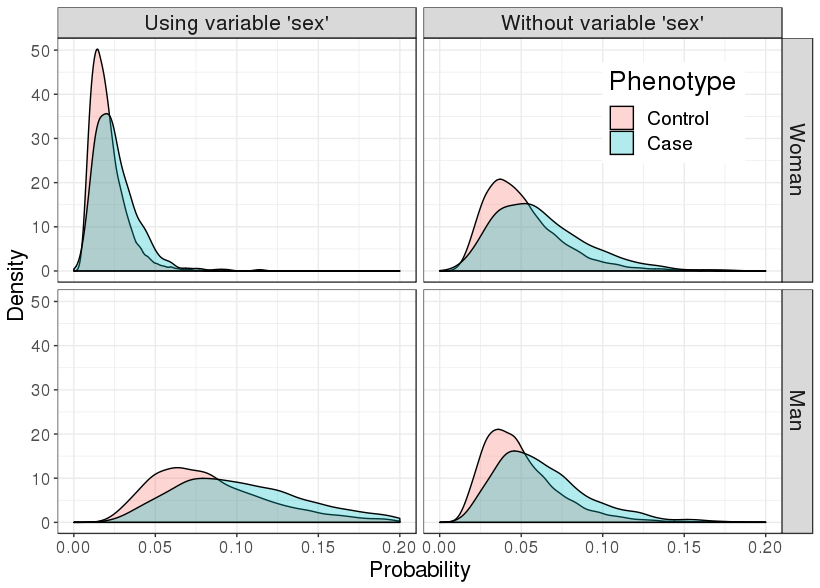
\includegraphics[width=0.8\textwidth]{dens-prob-CAD.png}}
\caption{Distribution of CAD predictions. Distribution of predicted probabilities of Coronary Artery Disease (CAD) in the UK Biobank using SCT. Upper / lower panels corresponds to women / men. Left panels correspond to a model using C+T scores and variable `sex' when fitting penalized logistic regression in the stacking step. Right panels correspond to performing stacking of C+T scores without using variable `sex'.}
\label{fig:sexCAD}
\end{figure}

%%%%%%%%%%%%%%%%%%%%%%%%%%%%%%%%%%%%%%%%%%%%%%%%%%%%%%%%%%%%%%%%%%%%%%%%%%%%%%%%

\clearpage

\vspace*{1em}

% latex table generated in R 3.5.2 by xtable 1.8-4 package
% Tue May 21 19:07:57 2019
\begin{table}[!htpb]
\centering
\begin{tabular}{|l|c|c|c|c|c|}
  \hline
Scenario & stdCT & maxCT & SCT & lassosum & LDpred \\ 
  \hline
100 & 82.0 [81.6-82.5] & 86.8 [86.4-87.2] & 86.1 [85.7-86.5] & 83.9 [83.5-84.4] & 76.3 [75.7-77.0] \\ 
  10K & 72.4 [71.5-73.5] & 75.6 [75.1-76.1] & 76.4 [75.9-77.0] & 75.0 [74.4-75.7] & 71.2 [70.6-71.9] \\ 
  1M & 68.7 [68.1-69.2] & 69.0 [68.3-69.6] & 69.1 [68.6-69.6] & 70.1 [69.5-70.6] & 71.0 [70.3-71.6] \\ 
  2chr & 77.4 [76.9-78.0] & 78.8 [78.3-79.4] & 82.1 [81.6-82.7] & 79.0 [78.3-79.8] & 74.6 [73.6-75.8] \\ 
  err & 70.1 [69.3-70.9] & 70.9 [70.5-71.5] & 73.4 [72.8-74.1] & 72.0 [71.3-72.9] & 70.7 [70.1-71.4] \\ 
  HLA & 78.7 [78.0-79.5] & 79.8 [79.2-80.3] & 80.7 [80.2-81.3] & 79.4 [78.7-80.2] & 76.9 [76.3-77.4] \\ 
   \hline
\end{tabular}
\caption{Results of the 6 simulation scenarios with well imputed variants. Scenarios are (100) 100 random causal variants; (10K) 10,000 random causal variants; (1M) all 1M variants are causal variants; (2chr) 100 variants of chromosome 1 are causal and all variants of chromosome 2, with half of the heritability for both chromosomes; (err) 10,000 random causal variants, but 10\% of the GWAS effects are reported with an opposite effect; (HLA) 7105 causal variants in a long-range LD region of chromosome 6. Mean and 95\% CI of $10^4$ non-parametric bootstrap replicates of the mean AUC of 10 simulations for each scenario. These results are plotted in figure 1.\label{tab:AUC-simu1}}
\end{table}


\vspace*{6em}

\begin{table}[!htpb]
\centering
\begin{tabular}{|l|c|c|c|c|}
  \hline
Trait & stdCT & maxCT & SCT & lassosum \\
  \hline
Breast cancer (BRCA) & 62.1 [60.5-63.6] & 63.3 [61.7-64.8] & 65.9 [64.4-67.4] & 57.9 [56.3-59.5] \\
 & 6256 & 2572 & 670,050 & 322,003 \\
Rheumatoid arthritis (RA) & 59.8 [57.7-61.8] & 60.3 [58.3-62.4] & 61.3 [59.1-63.4] & 59.5 [57.5-61.7] \\
 & 12,220 & 88,556 & 317,456 & 672,922 \\
Type 1 diabetes (T1D) & 75.4 [72.4-78.4] & 76.9 [73.9-79.7] & 78.7 [75.7-81.7] & 75.3 [72.2-78.3] \\
 & 1112 & 267 & 135,991 & 204,785 \\
Type 2 diabetes (T2D) & 59.1 [58.1-60.1] & 60.7 [59.8-61.7] & 63.8 [62.9-64.7] & 63.2 [62.3-64.1] \\
 & 177 & 33,235 & 548,343 & 256,353 \\
Prostate cancer (PRCA) & 68.0 [66.5-69.5] & 69.3 [67.8-70.8] & 71.7 [70.2-73.1] & 58.7 [57.1-60.3] \\
 & 1035 & 356 & 696,575 & 121,660 \\
Depression (MDD) & 55.7 [54.4-56.9] & 59.2 [58.0-60.4] & 59.5 [58.2-60.7] & 52.0 [50.8-53.3] \\
 & 165,584 & 222,912 & 524,099 & 625,732 \\
Coronary artery disease (CAD) & 59.9 [58.6-61.2] & 61.1 [59.9-62.4] & 63.9 [62.7-65.1] & 63.0 [61.8-64.2] \\
 & 1182 & 87,577 & 315,165 & 290,204 \\
Asthma & 56.8 [56.2-57.5] & 57.3 [56.7-58.0] & 60.7 [60.0-61.3] & 58.7 [58.1-59.4] \\
 & 3034 & 360 & 446,120 & 75,965 \\
   \hline
\end{tabular}
\caption{Results of the real data applications with large training size.
AUC values on the test set of UKBB (mean [95\% CI] from $10^4$ bootstrap samples) and the number of variants used in the final model. Training SCT and choosing optimal hyper-parameters for C+T and lassosum use 63\%-90\% of the individuals reported in table 1. These results are plotted in figure 2.\label{tab:AUC}}
\end{table}

%%%%%%%%%%%%%%%%%%%%%%%%%%%%%%%%%%%%%%%%%%%%%%%%%%%%%%%%%%%%%%%%%%%%%%%%%%%%%%%%

% latex table generated in R 3.5.2 by xtable 1.8-4 package
% Wed Jun 19 15:19:38 2019
\begin{table}[!htpb]
\centering
\begin{tabular}{|l|c|c|c|c|}
\hline
Scenario & stdCT & maxCT & SCT & lassosum \\ 
\hline
100  & 77.4 [76.0-78.8] & 83.9 [83.4-84.4] & 83.1 [82.6-83.6] & 80.1 [79.5-80.8] \\ 
10K  & 69.4 [68.4-70.5] & 73.0 [72.5-73.4] & 72.9 [72.5-73.3] & 71.2 [70.6-71.7] \\ 
1M   & 64.0 [63.6-64.4] & 64.0 [63.6-64.4] & 62.7 [62.3-63.0] & 64.1 [63.3-64.8] \\ 
2chr & 70.0 [68.8-71.2] & 74.4 [73.6-75.2] & 78.5 [77.9-79.1] & 73.2 [72.5-73.8] \\ 
err  & 67.0 [66.0-68.1] & 68.6 [67.7-69.5] & 69.5 [68.9-70.1] & 65.6 [64.9-66.3] \\ 
HLA  & 74.8 [72.9-76.3] & 75.3 [73.5-76.9] & 76.4 [74.5-78.0] & 75.8 [74.2-77.2] \\ 
\hline
\end{tabular}
\caption{Results of the 6 simulation scenarios with less well imputed variants. AUC values on the test set for simulations with less well imputed variants (mean [95\% CI] from $10^4$ bootstrap samples). These results are plotted in figure \ref{fig:AUC-simu2}.\label{tab:AUC-simu2}}
\end{table}

\begin{table}[!htpb]
\centering
\begin{tabular}{|l|c|c|c|c|c|}
\hline
Trait & stdCT & maxCT & SCT & lassosum & LDpred \\ 
\hline
Breast cancer (BRCA) & 61.9 [61.8-62.0] & 62.9 [62.6-63.2] & 62.7 [62.4-63.1] & 57.8 [57.1-58.5] & 62.0 [62.0-62.1] \\ 
Rheumatoid arthritis (RA) & 59.1 [59.0-59.2] & 59.5 [59.3-59.7] & 59.6 [59.3-59.8] & 58.8 [58.2-59.3] & 59.8 [59.7-59.8] \\ 
Type 1 diabetes (T1D) & 75.4 [74.6-76.2] & 76.0 [75.1-77.0] & 78.4 [77.7-79.1] & 75.5 [74.7-76.2] & 75.5 [74.7-76.3] \\ 
Type 2 diabetes (T2D) & 59.6 [59.5-59.7] & 60.4 [60.2-60.7] & 60.9 [60.6-61.1] & 63.2 [62.9-63.5] & 61.0 [60.6-61.3] \\ 
Prostate cancer (PRCA) & 67.0 [66.8-67.2] & 68.5 [68.3-68.7] & 69.0 [68.5-69.4] & 57.1 [56.3-58.1] & 65.6 [65.5-65.7] \\ 
Depression (MDD) & 54.1 [53.7-54.4] & 58.7 [58.3-59.0] & 54.7 [54.4-55.0] & 52.9 [52.0-53.8] & 60.0 [60.0-60.1] \\ 
Coronary artery disease (CAD) & 59.7 [59.5-59.9] & 61.1 [60.6-61.5] & 60.8 [60.6-61.1] & 62.8 [62.6-62.9] & 61.0 [60.9-61.1] \\ 
Asthma & 56.3 [56.2-56.5] & 56.9 [56.8-56.9] & 56.3 [55.6-56.9] & 57.7 [57.3-58.0] & 56.5 [56.3-56.7] \\ 
\hline
\end{tabular}
\caption{Results of the real data applications with small training size. Mean and 95\% CI of $10^4$ non-parametric bootstrap replicates of the mean AUC of 6 random splits to define the training set. Training SCT and choosing optimal hyper-parameters for C+T, LDpred and lassosum use 500 cases and 2000 controls only. These results are plotted in figure \ref{fig:AUC-real-small}.\label{tab:AUC2}}
\end{table}

%%%%%%%%%%%%%%%%%%%%%%%%%%%%%%%%%%%%%%%%%%%%%%%%%%%%%%%%%%%%%%%%%%%%%%%%%%%%%%%%

\clearpage
\subsection*{Caution on using covariates}

For example, because prevalence of CAD is much higher in men than in women in the UKBB (8-9\% vs 2\%), adding sex in the model amount to fitting two different intercepts, centering distributions of fitted probabilities around disease prevalence (Figure \ref{fig:sexCAD}). This increases the AUC from 63.9\% to 74.4\% but results in a model that would classify all women as healthy. A possible solution would be to report AUC figures for each gender separately, or even to fit a model for each gender separately (in the stacking step).
Fitting models separately would enable the use of sex chromosomes without introducing bias.
As for ancestry concerns, fitting different models for different ancestries might be a way to get more calibrated results and to account for differences in effect sizes and LD.
However, here for CAD, fitting two separate models for each gender results in a slight loss of predictive performance, while using variable `sex' does not change results when they are reported for each gender separately, with an AUC of 64.9\% [63.5-66.3] for men and 62.5\% [59.8-65.2] for women.
Thus, adding `sex' as a covariate in the model may provide a model with similar discrimination and with better calibration of probabilities (if prevalence in the data is representative of prevalence in the population). Yet, we would like to emphasize again that reporting one AUC figure for all individuals would be misleading in the case of using variable `sex' in the model.


\vspace*{6em}

\bibliographystyle{ajhg}
\bibliography{refs}

\end{document}
